\documentclass[conference]{IEEEtran}
\IEEEoverridecommandlockouts

\newif\ifanonymous
\anonymousfalse

\usepackage[utf8]{inputenc}
\usepackage[T1]{fontenc}
\usepackage{mathptmx}
\usepackage{amsmath,amssymb,amsfonts}
\usepackage{graphicx}
\usepackage{booktabs}
\usepackage{tabularx}
\usepackage{array}
\usepackage{xcolor}
\usepackage{hyperref}
\usepackage{cite}
\usepackage{microtype}
\usepackage{tikz}
\usepackage{pgfplots}
\pgfplotsset{compat=1.18}
\usetikzlibrary{arrows.meta,shapes,positioning,calc,fit,automata}
\setlength{\emergencystretch}{2.5em}
\hyphenation{wire-less cre-den-tial ESP-NOW}

\definecolor{ieeeBlue}{RGB}{27,54,93}
\definecolor{wsBlue}{RGB}{0,82,204}
\definecolor{wsLightBlue}{RGB}{238,246,255}
\definecolor{wsRed}{RGB}{180,20,18}
\definecolor{wsLightRed}{RGB}{255,248,246}
\definecolor{termBg}{RGB}{18,24,36}
\definecolor{termGreen}{RGB}{52,211,153}
\definecolor{termAmber}{RGB}{251,191,36}
\definecolor{termRed}{RGB}{248,113,113}
\definecolor{tealPlot}{RGB}{0,137,123}
\definecolor{greenPlot}{RGB}{46,125,50}
\definecolor{orangePlot}{RGB}{230,126,34}
\definecolor{purplePlot}{RGB}{106,27,154}

\ifanonymous
\hypersetup{colorlinks=true,linkcolor=ieeeBlue,citecolor=ieeeBlue,urlcolor=ieeeBlue,
pdftitle={CEE-PEW: A Layered Cryptographic Architecture for Securing ESP-NOW Edge Communication},
pdfauthor={Anonymous Author(s)},
pdfkeywords={ESP-NOW, ESP32, lightweight cryptography, Ascon-128, Ed25519, replay protection, BLE pairing}}
\else
\hypersetup{colorlinks=true,linkcolor=ieeeBlue,citecolor=ieeeBlue,urlcolor=ieeeBlue,
pdftitle={CEE-PEW: A Layered Cryptographic Architecture for Securing ESP-NOW Edge Communication},
pdfauthor={Rishi Misra and Anis Fatema},
pdfkeywords={ESP-NOW, ESP32, lightweight cryptography, Ascon-128, Ed25519, replay protection, BLE pairing}}
\fi

\setlength{\textfloatsep}{4pt plus 1pt minus 1pt}
\setlength{\floatsep}{4pt plus 1pt minus 1pt}
\setlength{\intextsep}{4pt plus 1pt minus 1pt}
\setlength{\abovecaptionskip}{2pt}
\setlength{\belowcaptionskip}{1pt}
\renewcommand{\arraystretch}{0.96}
\setcounter{topnumber}{4}
\setcounter{dbltopnumber}{2}
\renewcommand{\topfraction}{0.93}
\renewcommand{\dbltopfraction}{0.93}
\renewcommand{\textfraction}{0.05}
\renewcommand{\floatpagefraction}{0.88}
\renewcommand{\dblfloatpagefraction}{0.88}

\title{\large\textbf{CEE-PEW: A Layered Cryptographic Architecture for Securing ESP-NOW Edge Communication}}

\ifanonymous
\author{%
\IEEEauthorblockN{Anonymous Author(s)}%
\IEEEauthorblockA{Paper submitted for Double-Blind Peer Review at IEEE ICITIIT 2027\\
Source Code, Lua Dissector \& PCAP Artifacts: \textit{[Anonymized Repository for Blind Review]}}%
}
\else
\author{%
\IEEEauthorblockN{Rishi Misra}%
\IEEEauthorblockA{\textit{School of Electronics Engineering (SENSE)}\\
\textit{Vellore Institute of Technology}, Vellore, Tamil Nadu, India\\
\texttt{rishi.misra2025@vitstudent.ac.in}}%
\and
\IEEEauthorblockN{Anis Fatema}%
\IEEEauthorblockA{\textit{School of Electronics Engineering (SENSE)}\\
\textit{Vellore Institute of Technology}, Vellore, Tamil Nadu, India\\
\texttt{anis.fatema@vit.ac.in}}%
}
\fi

\date{}

\begin{document}
\maketitle

\begin{abstract}
\textit{(1) Research Problem.} Connectionless ESP-NOW links carry low-latency traffic between ESP32 nodes without access-point infrastructure. However, receive-side CCMP enforcement was not established for the evaluated ESP-IDF driver configuration (GitHub Issue \#15179), caps hardware-encrypted peers at 17, and in middleware revisions prior to v2.5.2 admitted 32-slot cache-eviction replay (CVE-2024-42483).
\textit{(2) Proposed Architecture.} Cryptographic End-to-End Peer-to-peer Encrypted Wireless (CEE-PEW) treats ESP-NOW strictly as an untrusted transport on dual-core ESP32 hardware costing under US\$28/pair. It executes out-of-band BLE commitment pairing, complete BLE stack teardown, Wi-Fi station bring-up, and in-band X25519 re-keying in sequence, backed by a 48\,KB static bump allocator with zero application-layer heap allocation ($\Delta_{\text{heap,app}} = 0$\,B).
\textit{(3) Implementation \& Methodology.} Under the 250\,B ESP-NOW v1.0 ceiling, we define and evaluate three explicit configurations: a \textbf{shipping Full profile without FEC (187\,B wire frame)}, an \textbf{experimental FEC-enabled Full ablation profile (249\,B wire frame)}, and an \textbf{AEAD-only Lite profile without FEC (105\,B wire frame)}. Evaluation combines a 17-suite ASan/UBSan host harness with a sealed two-node hardware timing rig at 160\,MHz and a third independent promiscuous sniffer.
\textit{(4) Principal Quantitative Findings.} On the host harness, 100/100 injected replay vectors across four fault classes and 24/24 header-tamper vectors were rejected. On hardware, compact 64-bit-limb TweetNaCl Ed25519 verification requires a median of 663.281\,ms (95\% CI $[663.200, 663.332]$\,ms, $N=50$), bounding Full-profile receive goodput to 74--88\,B/s (or 44\,B/s when a retransmitted duplicate is verified twice), whereas symmetric Ascon-128 v1.2 encryption takes 0.12\,ms. Across bidirectional runs, MAC-layer send callbacks reported 100\% completion while application-layer reassembly reached 91.7--92.1\% ($\approx 8$\,pp lower). A Hamming(15,11) FEC ablation over a 1\,m LOS link corrected 0 single-bit errors across 97--99 fragments with indistinguishable delivery (94.3\% vs.\ 93.8\%), motivating its removal from the shipping build.
\textit{(5) Disclosed Limitations.} The 663.3\,ms bottleneck reflects our unwindowed 64-bit-limb TweetNaCl port rather than an inherent ESP32 architectural limit. The 4-character pairing code provides transcript consistency but does not resist offline dictionary enumeration of captured SHA-256 commitments. Delivery provides MAC-acknowledged transmission with receiver-side duplicate suppression rather than application-layer at-least-once guarantees. Finally, nine-channel frequency hopping was designed but disabled in all evaluated builds.
\end{abstract}

\textit{AI assistance:} The authors used AI tools for language editing and clarity. All technical content, firmware, and measurements were verified by the authors.

\begin{IEEEkeywords}
Ascon-128 v1.2, authenticated encryption, CVE-2024-42483, edge cryptography, ESP32, ESP-NOW, IEEE 802.11 action frames, IoT security, replay protection, X25519.
\end{IEEEkeywords}

\section{Introduction}
Cellular coverage and access-point backhaul are both absent in off-grid industrial and robotic deployments, leaving an infrastructure-free radio link as the primary option~\cite{montiel2026}. ESP-NOW~\cite{espressif_espnow} dispenses with Wi-Fi association and the TCP/IP stack altogether, encapsulating each payload inside an IEEE 802.11 vendor-specific management action frame (\texttt{subtype 0x00d0}, OUI \texttt{18:fe:34}) transmitted at $1$\,Mbps. Frame capacity depends on the SDK revision: ESP-NOW v2.0 (available from ESP-IDF v5.4.2 onward) lifts the ceiling to $1{,}470$\,B~\cite{espressif_espnow}, whereas the v1.0 limit of $250$\,B still binds ESP-IDF v4.x and ESP8266-SDK nodes, and Espressif advises $\le 250$\,B wherever a network mixes revisions. At $1$\,Mbps with a long PLCP preamble, a full v1.0 frame occupies $2.528$\,ms of computed physical airtime ($288$\,B MPDU, $4$\,B FCS, and $192\,\mu$s PLCP), governing collision probability on an uncoordinated 2.4\,GHz link without RTS/CTS.

Smart-home automation~\cite{cujilema2023} and multi-agent swarm robotics~\cite{caniago2026} have both adopted ESP-NOW widely. Yet, five structural limitations affect security layers built directly on the native driver or middleware.
\begin{enumerate}
\setlength{\itemsep}{0pt}\setlength{\parskip}{0pt}
\item \textit{Unverified receive-side CCMP in the evaluated driver.} Receive-side CCMP enforcement was not established for the evaluated ESP-IDF driver configuration, motivating independent application-layer authentication. Inside the core driver, a receiver configured for CCMP encryption accepted unencrypted frames spoofed with a peer's MAC address. The issue remains open in Espressif's tracker (Issue \#15179, last verified activity Jan.\ 2025)~\cite{espressif_issue15179}.
\item \textit{Replay and memory-safety defects in middleware (CVE-2024-42483 / CVE-2024-42484):} Two flaws affected Espressif's \texttt{esp-now} middleware component before v2.5.2, disclosed on Sept.\ 10 2024~\cite{nozomi2024,nvd_cve42483}. CVE-2024-42483 permitted verbatim replay even under active CCMP or application-layer AES-CCM because transmitting 32 frames evicted a shared 32-slot circular cache of 16-bit magic fields. CVE-2024-42484 was an out-of-bounds read enabling remote crash or denial of service. Additionally, links built directly on the bare ESP-IDF \texttt{esp\_now} API inherit no sequence cache of any kind.
\item \textit{Static keying and no forward secrecy:} Native CCMP and the \texttt{esp-now} AES-128-CCM path rely on static keys (PMK or LMK) stored in flash. Compromising one node exposes every session, past and future.
\item \textit{Hardware peer-table exhaustion:} The ESP32 Wi-Fi hardware encryption key table admits at most 17 encrypted peers (7 by default)~\cite{espressif_espnow}, capping mesh fan-out. This ceiling restricts large swarms.
\item \textit{Fixed channel and fingerprintable OUI:} Frames transmit on a single fixed channel and expose Espressif's OUI header to wireless intrusion detection systems~\cite{guardianair2024}. The signature is easily recognized.
\end{enumerate}

To prevent ambiguity between the abstract, text, and experimental tables, we explicitly distinguish three wire-frame configurations evaluated for a worst-case $58$\,B compressed payload chunk ($|P_c|=58$\,B).
\begin{itemize}
\setlength{\itemsep}{0pt}\setlength{\parskip}{0pt}
\item \textbf{Shipping Configuration (CEE-PEW Full without FEC --- $187$\,B wire budget).} The default shipping build (\texttt{CONFIG\_CEEPEW\_FEC\_DISABLE=1}) combining static Huffman compression, inner Ascon-128 v1.2 AEAD, outer XSalsa20-HMAC-128 box encryption, per-fragment $64$\,B Ed25519 signature, $24$\,B Extended Security Layer (ESL) header, CRC-32, and $1$\,B ARQ sequence wrapper.
\item \textbf{Experimental FEC Ablation Configuration (CEE-PEW Full with FEC --- $249$\,B max wire frame):} Identical to the Full profile above, but inserting session-permuted Hamming(15,11) FEC ($+62$\,B parity and inner CRC overhead at $|P_c|=58$\,B), reaching $249$\,B right beneath the $250$\,B v1.0 limit.
\item \textbf{Lite Configuration (CEE-PEW Lite without FEC --- $105$\,B air payload; $138$\,B with FEC):} An AEAD-only profile for point-to-point sessions authenticated at pairing and PFS re-keying, omitting the outer box and per-fragment Ed25519 signature. Symmetric keys are established at pairing.
\end{itemize}

Rather than claiming new cryptographic primitives, our contribution lies in the engineering integration, sequential dual-radio lifecycle, and empirical trade-off evaluation on constrained ESP32 hardware.
\begin{enumerate}
\setlength{\itemsep}{0pt}\setlength{\parskip}{0pt}
\item \textbf{Sequential dual-radio lifecycle and heap-free engine.} A two-node prototype at under US\$28/pair separates BLE pairing from ESP-NOW transport in time and across cores, backed by a $48$\,KB static bump-allocator pool with zero application-layer heap allocation ($\Delta_{\text{heap,app}} = 0$\,B).
\item \textbf{Ephemeral key schedule and dual-mode framing:} Integration of X25519 key agreement~\cite{rfc7748}, domain-separated HKDF-SHA256~\cite{rfc5869}, inner Ascon-128 v1.2 AEAD~\cite{dobraunig2021}, an outer XSalsa20-HMAC-128 layer, and per-fragment Ed25519 signatures~\cite{bernstein2012} refreshed by an in-band PFS re-key, alongside the AEAD-only \textit{CEE-PEW Lite} profile.
\item \textbf{Cost-ordered RX and post-authentication replay commit:} Sender retransmission driven by the 802.11 MAC acknowledgement paired with inbound deduplication filtering and a 64-bit bounded sliding-bitmap replay window~\cite{donenfeld2017} that commits sequence numbers only after both the AD-bound Ascon tag and Ed25519 signature verify.
\item \textbf{Hardware cycle profiling and negative findings.} Measurements from a board pair pinned at $160$\,MHz ($N=80$ TX records/board, $N{=}97$--$99$ RX trials) isolate the $663.3$\,ms verification bottleneck to our 64-bit-limb TweetNaCl port. They demonstrate via controlled ablation that Hamming(15,11) FEC corrects zero errors over clean 802.11 FCS links, and disclose a $320$\,s epoch-shift defect in channel hopping.
\item \textbf{Multi-tier verification and open dissection artifacts:} $17$ ASan/UBSan host suites, $5$ libFuzzer harnesses, a $100$-vector host replay suite across four fault classes, a Wireshark Lua post-dissector (\path{ceepew_wireshark_dissector.lua}), and sealed PCAP captures.
\end{enumerate}

\begin{table*}[t]
\centering
\caption{Comparative Architectural and Security Positioning Across ESP-NOW and ESP32 Wireless Security Frameworks}
\label{tab:related_work}
\setlength{\tabcolsep}{3pt}
\scriptsize
\renewcommand{\arraystretch}{1.02}
\begin{tabularx}{\textwidth}{@{}>{\raggedright\arraybackslash}p{0.14\textwidth}>{\raggedright\arraybackslash}p{0.12\textwidth}>{\raggedright\arraybackslash}p{0.14\textwidth}>{\raggedright\arraybackslash}p{0.14\textwidth}X>{\raggedright\arraybackslash}p{0.14\textwidth}>{\raggedright\arraybackslash}p{0.10\textwidth}@{}}
\toprule
\textbf{System / Framework} & \textbf{Transport Link} & \textbf{Evaluation Environment} & \textbf{Key Agreement \& Forward Secrecy} & \textbf{Replay Defense \& RX Enforcement} & \textbf{Wire Frame ($58$\,B Chunk) / Goodput} & \textbf{Evidence Basis} \\
\midrule
Core ESP-IDF \texttt{esp\_now} CCMP~\cite{espressif_espnow,espressif_issue15179} & 802.11 Action (OUI \texttt{18:fe:34}) & ESP32 point-to-point link (SDK driver) & Static PMK/LMK ($\le 17$ peers); None & No built-in seq cache; unverified RX~\cite{espressif_issue15179} & $74$\,B ($+16$\,B CCMP); $\le 250$\,B v1.0 & Spec + Computed airtime \\
Espressif \texttt{esp-now} AES-CCM~\cite{nozomi2024,nvd_cve42483} & ESP-NOW Middleware & ESP32 application middleware & Static / ECDH provisioning; None & 32-slot cache (CVE-2024-42483 pre-v2.5.2) & $\approx 86$\,B est.\ (App AES-128-CCM) & Estimated from advisory~\cite{nozomi2024} \\
\texttt{SecurePair} (ESP-NOW/LoRa)~\cite{securepair2026} & ESP-NOW or LoRa & Arduino / ESP32 standalone library & Ephemeral X25519 (LED/OTA); Session-level & Monotonic counter; dynamic Arduino heap alloc & $\approx 90$\,B est.\ (AES-256-GCM); no BLE/PFS re-key & Estimated from source \\
ESP-NOW Swarm / Mesh~\cite{caniago2026} & ESP-NOW / Wi-Fi Mesh & Multi-robot indoor navigation & None at message layer; None & None (cleartext JSON/struct payloads) & $58$\,B ($0$\,B crypto overhead) & Measured OTA (cleartext) \\
ESP32--MQTT--Pi~\cite{setiawan2021,amirkhanova2026} & Wi-Fi TCP/IP (MQTT Broker) & ESP32 client to Raspberry Pi broker & Static pre-shared key; None & None in CBC~\cite{setiawan2021} / App seq~\cite{amirkhanova2026} & TCP/IP MTU ($+16\text{--}28$\,B AES, $+20\text{--}30$\,ms) & Measured over Wi-Fi AP \\
\textbf{CEE-PEW Lite} \textit{(This Work)} & ESP-NOW (Ch.\ 1 fixed in eval.) & 2$\times$ ESP32 DevKit v1 (160\,MHz, 20\,cm LOS) & Ephemeral X25519 (BLE+PFS re-key) & 64-b parity nonce + sliding bitmap; 0\,B app heap & $\mathbf{105\,\textbf{B}}$ no FEC ($138$\,B FEC); $\approx \mathbf{2.1\,\textbf{KB/s}}$ & \textbf{Measured HW + Host KAT} \\
\textbf{CEE-PEW Full} \textit{(This Work)} & ESP-NOW (Ch.\ 1 fixed in eval.) & 2$\times$ ESP32 DevKit v1 (160\,MHz, 20\,cm LOS) & Ephemeral X25519 (BLE+PFS re-key) & 64-b parity nonce + sliding bitmap + Ed25519 & $\mathbf{187\,\textbf{B}}$ ship ($249$\,B FEC); $74\text{--}88$\,B/s ($44$\,B/s dup) & \textbf{Measured HW + Host KAT} \\
\bottomrule
\end{tabularx}
\end{table*}

\section{Related Work}
Table~\ref{tab:related_work} positions CEE-PEW against existing ESP-NOW and ESP32 security frameworks, explicitly identifying each system's evaluation environment and distinguishing measured hardware values from analytical estimates. Static-keyed AES-256-GCM over MQTT was measured by Amirkhanova et al.~\cite{amirkhanova2026} at $\approx 30$\,ms latency, while AES-256-CBC was checked against NIST vectors by Setiawan and Magfirawaty~\cite{setiawan2021} with no authentication or replay checking and $\approx 20$\,ms overhead; both systems sit behind a Wi-Fi access point and an MQTT broker. Ascon-128 v1.2 was introduced by Dobraunig et al.~\cite{dobraunig2021}, selected as the CAESAR primary choice for lightweight applications, and standardized by NIST in SP~800-232~\cite{nist_ascon2025}. The AEAD benchmarking protocol of Atul et al.~\cite{atul2026} is an unrefereed ePrint preprint containing no hardware measurements. Their results lack on-device benchmarks.

Connectionless ESP-NOW links measured in the field report $>92\%$ indoor delivery and $\approx 2.4$\,ms single-hop latency at $1$\,Mbps for unencrypted payloads~\cite{urazayev2023,caniago2026,montiel2026}. Cujilema Paguay et al.~\cite{cujilema2023} added static-key AES to ESP-NOW, while Espressif's \texttt{esp-now} middleware introduced AES-128-CCM and was patched in v2.5.2 after CVE-2024-42483/42484~\cite{nozomi2024,nvd_cve42483}. \texttt{SecurePair}~\cite{securepair2026} pairs X25519 with AES-256-GCM using dynamic allocations. Albrecht et al.~\cite{albrecht2021} documented the failure of mesh messaging without sender authentication (Bridgefy), motivating explicit identity binding and replay tracking. Because these prior systems operate under disparate environments and omit per-stage MCU cycle breakdowns, Table~\ref{tab:related_work} is presented as an architectural comparison rather than a controlled latency benchmark.

\begin{figure*}[t]
\centering
\includegraphics[width=0.84\textwidth]{ceepew_hardware_prototype_fig.pdf}
\caption{CEE-PEW hardware ($<$US\$28/pair): ESP32-WROOM-32 with SSD1306 OLED (\texttt{GPIO26/27}), potentiometer (\texttt{GPIO33}), button (\texttt{GPIO19}), RGB LED (\texttt{GPIO15/18/23}), and diagnostic switch (\texttt{GPIO5}). (a)~Circuit pinout and schematic; (b)~the assembled breadboard node.}
\label{fig:hardware_proto}
\end{figure*}

\section{System Architecture and Memory Model}

\subsection{Hardware Platform and Sequential Dual-Radio Lifecycle}
Every node is an ESP32-WROOM-32 DevKit v1 (Fig.~\ref{fig:hardware_proto}). The board supplies a $128\times 64$ SSD1306 I$^2$C OLED, a $10\,\text{k}\Omega$ rotary potentiometer filtered by an exponential moving average ($\alpha = 0.25$), a software-debounced tactile confirm button, an RGB status LED, and a hardware diagnostic switch; a pair of finished nodes costs Rs.\,1,566--2,312 ($\approx$US\$19--28) with no companion smartphone. Because \texttt{GPIO15} (RGB LED) and \texttt{GPIO5} (diagnostic switch) are ESP32 boot strapping pins, the circuit leaves both at their default logic levels during reset.

Because the ESP32 shares a single 2.4\,GHz RF front-end and antenna between Bluetooth and Wi-Fi, concurrent BLE scanning and ESP-NOW transmission suffer severe coexistence arbitration losses. CEE-PEW grants exclusive radio ownership to one stack at a time across three sequential phases (Fig.~\ref{fig:session_fsm}):
\begin{itemize}
\setlength{\itemsep}{0pt}\setlength{\parskip}{0pt}
\item \textbf{Phase 1 (BLE Discovery):} Both nodes generate ephemeral X25519 and Ed25519 keypairs using the hardware TRNG (\texttt{esp\_random()}). The first $16$ bytes of a $32$-byte SHA-256 commitment and a $2$-byte monotonic nonce ride in a $31$-byte BLE scan response. The lower 6-byte MAC becomes the initiator.
\item \textbf{Phase 2 (GATT Pairing \& Local Code Confirmation):} Over BLE GATT each peer sends its Ed25519 and X25519 public keys and Wi-Fi STA MAC encrypted under a transient Ascon-128 v1.2 AEAD bootstrap key derived via HKDF from the user-entered $4$-character code and peer BLE MACs (purged and zeroized immediately upon BLE teardown). Both OLEDs display the full $32$-byte commitment beside the $4$-character code; a button press within $45$\,s confirms transcript match.
\item \textbf{Phase 3 (BLE Teardown, Rendezvous \& PFS Session):} After exchanging handoff beacons, both nodes completely disable and deinitialize Bluedroid and the BLE controller before bringing up Wi-Fi STA and ESP-NOW on Channel~1. A $5$\,B/$9$\,B Rendezvous exchange aligns node uptimes, followed by a $1$\,B handshake barrier verifying bidirectional decryption. An in-band \textbf{Perfect Forward Secrecy (PFS) re-key} ($77$\,B frame, authenticated by HMAC-SHA256 under the pairing secret) installs a fresh X25519 session key and zeroizes prior keys via \texttt{ceepew\_secure\_zero()}. Nine-channel frequency hopping was designed but disabled in all evaluated builds (\texttt{CONFIG\_CEEPEW\_CHANNEL\_HOP=0}), fixing both radios to Channel~1 (Section~\ref{sec:hop-disabled}).
\end{itemize}

\subsection{Dual-Core Concurrency and Application-Level Static Memory}
The firmware runs on ESP-IDF v6.0.3 under FreeRTOS ($1{,}000$\,Hz tick) across both Xtensa LX6 cores. Core~0 runs the $60$\,Hz UI loop (\texttt{task\_ui}, $10{,}240$\,B stack), while Core~1 runs the session FSM, cryptographic pipeline, and radio callbacks (\texttt{task\_session}, $16{,}384$\,B stack). An 8-deep UI event queue ($28$\,B \texttt{UIEvent\_t}) and a 32-deep session RX queue (\texttt{g\_session\_rx\_queue}) handle inter-core IPC. Transient pipeline buffers come from a compile-time $48$\,KB 8-byte-aligned static pool in \texttt{.bss} whose bump allocator zeroes and resets after each message, guaranteeing \textbf{zero application-level heap allocation} ($\Delta_{\text{heap,app}} = 0$\,B; the underlying mbedTLS PSA, BLE, and Wi-Fi stacks still allocate internally during init).

\section{Implementation}

\subsection{Static Region Memory and Stage Pipelines}
Allocation is a bump of a $32$-bit offset rounded to an $8$-byte boundary across a table of $256$ extents. Nothing is freed piecemeal: \texttt{region\_reset()} enters a critical section, securely zeroes the entire $48$\,KB pool, and resets the bump pointer and table. Peak session demand is tracked via the bump pointer and a high-water mark. Memory bounds are strictly enforced. (HWM).

\begin{figure}[t]
\centering
\resizebox{\columnwidth}{!}{%
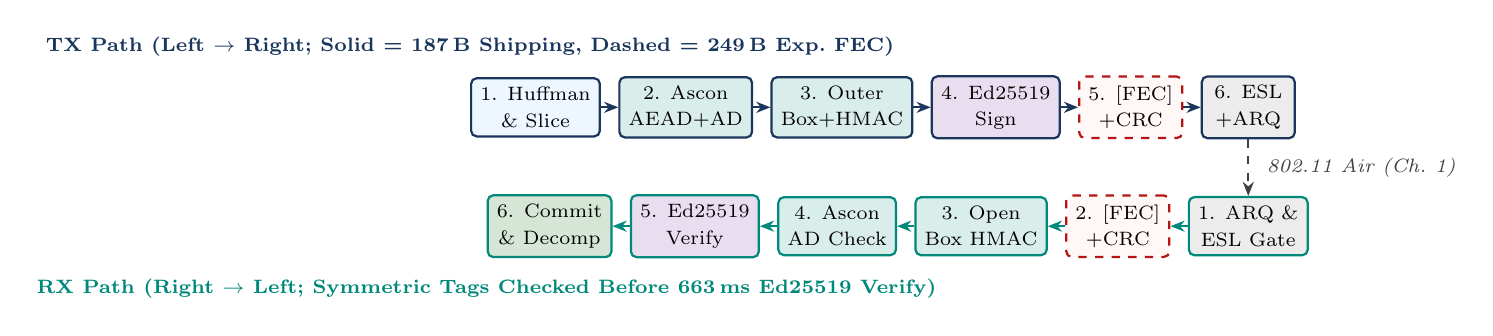
\begin{tikzpicture}[
  node distance=0.22cm and 0.22cm,
  block/.style={rectangle, draw=ieeeBlue, thick, rounded corners=2pt, font=\scriptsize, align=center, minimum width=1.18cm, minimum height=0.62cm},
  fecblock/.style={rectangle, draw=wsRed, thick, dashed, rounded corners=2pt, fill=wsLightRed, font=\scriptsize, align=center, minimum width=1.18cm, minimum height=0.62cm},
  arrow/.style={-{Stealth[length=1.8mm,width=1.4mm]}, thick, draw=ieeeBlue},
  rxarrow/.style={-{Stealth[length=1.8mm,width=1.4mm]}, thick, draw=tealPlot}
]
% TX Row
\node[block, fill=wsLightBlue] (huff) {1. Huffman\\[1.5pt]\& Slice};
\node[block, right=of huff, fill=tealPlot!15] (aead) {2. Ascon\\[1.5pt]AEAD+AD};
\node[block, right=of aead, fill=tealPlot!15] (box) {3. Outer\\[1.5pt]Box+HMAC};
\node[block, right=of box, fill=purplePlot!15] (sig) {4. Ed25519\\[1.5pt]Sign};
\node[fecblock, right=of sig] (fec) {5. [FEC]\\[1.5pt]+CRC};
\node[block, right=of fec, fill=gray!15] (esl) {6. ESL\\[1.5pt]+ARQ};

% RX Row (below TX)
\node[block, below=0.72cm of esl, fill=gray!15, draw=tealPlot] (rxesl) {1. ARQ \&\\[1.5pt]ESL Gate};
\node[fecblock, left=of rxesl] (rxfec) {2. [FEC]\\[1.5pt]+CRC};
\node[block, left=of rxfec, fill=tealPlot!15, draw=tealPlot] (rxbox) {3. Open\\[1.5pt]Box HMAC};
\node[block, left=of rxbox, fill=tealPlot!15, draw=tealPlot] (rxaead) {4. Ascon\\[1.5pt]AD Check};
\node[block, left=of rxaead, fill=purplePlot!15, draw=tealPlot] (rxsig) {5. Ed25519\\[1.5pt]Verify};
\node[block, left=of rxsig, fill=greenPlot!20, draw=tealPlot] (rxdec) {6. Commit\\[1.5pt]\& Decomp};

% TX Arrows
\draw[arrow] (huff) -- (aead);
\draw[arrow] (aead) -- (box);
\draw[arrow] (box) -- (sig);
\draw[arrow] (sig) -- (fec);
\draw[arrow] (fec) -- (esl);

% Air Hop: label cleanly positioned to the right of the downward arrow
\draw[arrow, dashed, draw=darkgray] (esl.south) -- node[right=3pt, font=\scriptsize\itshape, text=darkgray] {802.11 Air (Ch.\ 1)} (rxesl.north);

% RX Arrows
\draw[rxarrow] (rxesl) -- (rxfec);
\draw[rxarrow] (rxfec) -- (rxbox);
\draw[rxarrow] (rxbox) -- (rxaead);
\draw[rxarrow] (rxaead) -- (rxsig);
\draw[rxarrow] (rxsig) -- (rxdec);

% Symmetrically aligned labels with comfortable 4pt padding
\node[font=\scriptsize\bfseries, text=ieeeBlue, anchor=west] at (huff.north west) [above=4pt] {TX Path (Left $\rightarrow$ Right; Solid = 187\,B Shipping, Dashed = 249\,B Exp.\ FEC)};
\node[font=\scriptsize\bfseries, text=tealPlot, anchor=west] at (rxdec.south west) [below=4pt] {RX Path (Right $\rightarrow$ Left; Symmetric Tags Checked Before 663\,ms Ed25519 Verify)};
\end{tikzpicture}%
}
\caption{CEE-PEW transmit and receive stage pipeline inside the 48\,KB static region pool ($\Delta_{\text{heap,app}}=0$\,B). Dashed blocks denote the experimental Hamming(15,11) FEC stage compiled out of the 187\,B shipping configuration.}
\label{fig:pipeline}
\end{figure}

\begin{figure}[t]
\centering
\resizebox{\columnwidth}{!}{%
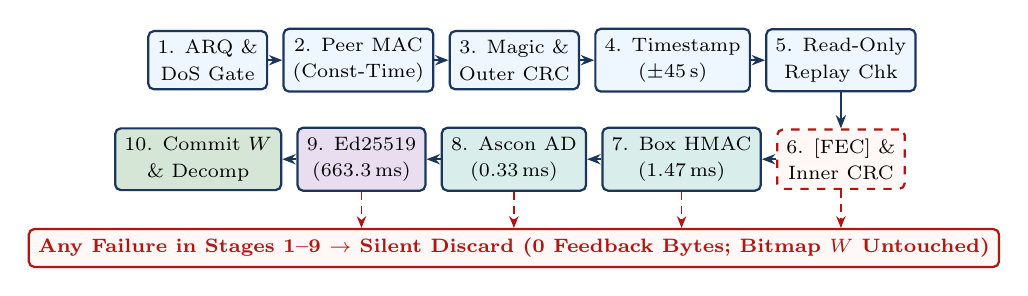
\begin{tikzpicture}[
  node distance=0.38cm and 0.18cm,
  block/.style={rectangle, draw=ieeeBlue, thick, rounded corners=2pt, font=\scriptsize, align=center, minimum width=1.22cm, minimum height=0.58cm},
  fecblock/.style={rectangle, draw=wsRed, thick, dashed, rounded corners=2pt, fill=wsLightRed, font=\scriptsize, align=center, minimum width=1.22cm, minimum height=0.58cm},
  dropblock/.style={rectangle, draw=wsRed, thick, rounded corners=2pt, fill=wsLightRed, font=\scriptsize\bfseries, text=wsRed, align=center, minimum width=7.4cm, minimum height=0.46cm},
  arrow/.style={-{Stealth[length=1.7mm,width=1.3mm]}, thick, draw=ieeeBlue},
  droparrow/.style={-{Stealth[length=1.5mm,width=1.2mm]}, semithick, densely dashed, draw=wsRed}
]
% Row 1: Pre-auth header checks (stages 1-5)
\node[block, fill=wsLightBlue] (arq) {1. ARQ \&\\[1.5pt]DoS Gate};
\node[block, right=of arq, fill=wsLightBlue] (mac) {2. Peer MAC\\[1.5pt](Const-Time)};
\node[block, right=of mac, fill=wsLightBlue] (crc) {3. Magic \&\\[1.5pt]Outer CRC};
\node[block, right=of crc, fill=wsLightBlue] (ts) {4. Timestamp\\[1.5pt]($\pm 45$\,s)};
\node[block, right=of ts, fill=wsLightBlue] (rep) {5. Read-Only\\[1.5pt]Replay Chk};

% Row 2: Crypto & Commit (stages 6-10, right to left)
\node[fecblock, below=0.46cm of rep] (fecdec) {6. [FEC] \&\\[1.5pt]Inner CRC};
\node[block, left=of fecdec, fill=tealPlot!15] (boxdec) {7. Box HMAC\\[1.5pt]($1.47$\,ms)};
\node[block, left=of boxdec, fill=tealPlot!15] (ascon) {8. Ascon AD\\[1.5pt]($0.33$\,ms)};
\node[block, left=of ascon, fill=purplePlot!15] (sigv) {9. Ed25519\\[1.5pt]($663.3$\,ms)};
\node[block, left=of sigv, fill=greenPlot!20] (commit) {10. Commit $W$\\[1.5pt]\& Decomp};

% Row 3: Silent Discard Bar (centred under ascon)
\node[dropblock, below=0.46cm of ascon] (discard) {Any Failure in Stages 1--9 $\rightarrow$ Silent Discard (0 Feedback Bytes; Bitmap $W$ Untouched)};

% Flow Arrows
\draw[arrow] (arq) -- (mac);
\draw[arrow] (mac) -- (crc);
\draw[arrow] (crc) -- (ts);
\draw[arrow] (ts) -- (rep);
\draw[arrow] (rep.south) -- (fecdec.north);
\draw[arrow] (fecdec) -- (boxdec);
\draw[arrow] (boxdec) -- (ascon);
\draw[arrow] (ascon) -- (sigv);
\draw[arrow] (sigv) -- (commit);

% Direct vertical drop arrows from the 4 verification stages into the discard bar
\draw[droparrow] (fecdec.south) -- (fecdec.south |- discard.north);
\draw[droparrow] (boxdec.south) -- (boxdec.south |- discard.north);
\draw[droparrow] (ascon.south) -- (ascon.south |- discard.north);
\draw[droparrow] (sigv.south) -- (sigv.south |- discard.north);
\end{tikzpicture}%
}
\caption{Cost-ordered receive-path flowchart: bounded header checks (Stages 1--5) and symmetric authenticators (Stages 7--8) run ahead of Ed25519 verification (Stage 9). Replay bitmap $W$ commits at Stage 10 only after both the AD-bound Ascon tag and Ed25519 signature verify.}
\label{fig:receive_path}
\end{figure}

The pipeline is an array of up to $16$ stages (\texttt{CEEPEW\_PIPELINE\_MAX\_STAGES}) sharing the uniform signature \texttt{(region, in, in\_len, out, out\_len, ctx)}. Fig.~\ref{fig:pipeline} shows the TX and RX paths, while Fig.~\ref{fig:receive_path} details the ten-stage cost-ordered receive flow. All memory is statically bounded.

\subsection{Session Lifecycle and Handoff Ordering}
The session state machine defines \texttt{IDLE}, \texttt{DISCOVERY}, \texttt{COMMITMENT}, \texttt{GATT\_IDENTITY}, \texttt{KEY\_DERIVE}, \texttt{POST\_DERIVE\_SYNC}, and \texttt{ACTIVE}, with \texttt{FAILED} as the terminal fail-closed state (Fig.~\ref{fig:session_fsm}). Timeouts enforce liveness: $30$\,s for discovery, $45$\,s for GATT identity and local PIN confirmation, $50$\,s for key derivation and radio teardown, and $30$\,s for the post-derive barrier. Fig.~\ref{fig:pairing_seq} illustrates the five-step pairing and handoff sequence. Measured from \texttt{PFS\_REQ} transmission to the first application frame, the in-band X25519 re-key takes $4.09$--$4.47$\,s of wall-clock time on hardware (covering key generation and ECDH on both nodes, radio transmission, MAC-ACK waits, ARQ backoff, and mutex scheduling). If the peer's Ed25519 public key never arrives or commitments mismatch, pairing aborts fail-closed without deriving a session key.

\begin{figure}[t]
\centering
\resizebox{\columnwidth}{!}{%
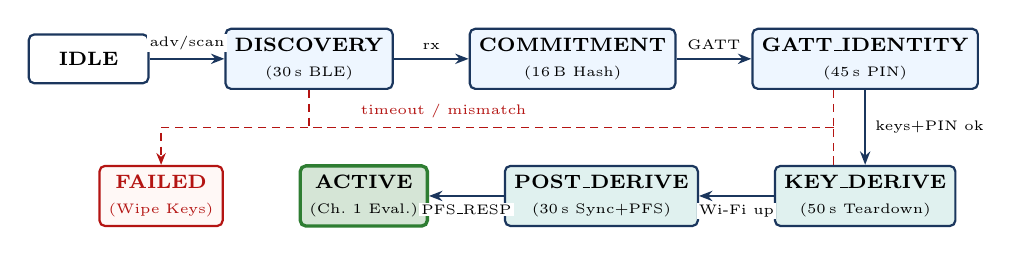
\begin{tikzpicture}[
  node distance=0.85cm and 0.95cm,
  state/.style={rectangle, rounded corners=2pt, draw=ieeeBlue, thick, fill=wsLightBlue, minimum width=1.52cm, minimum height=0.62cm, font=\scriptsize\bfseries, align=center},
  actstate/.style={rectangle, rounded corners=2pt, draw=greenPlot, very thick, fill=greenPlot!20, minimum width=1.52cm, minimum height=0.62cm, font=\scriptsize\bfseries, align=center},
  failstate/.style={rectangle, rounded corners=2pt, draw=wsRed, thick, fill=wsLightRed, minimum width=1.52cm, minimum height=0.62cm, font=\scriptsize\bfseries, text=wsRed, align=center},
  arrow/.style={-{Stealth[length=1.7mm,width=1.3mm]}, thick, draw=ieeeBlue},
  failarrow/.style={-{Stealth[length=1.5mm,width=1.2mm]}, semithick, densely dashed, draw=wsRed}
]
% Top Row (BLE Ownership)
\node[state, fill=white] (idle) {IDLE};
\node[state, right=of idle] (disc) {DISCOVERY\\[1pt]\normalfont\tiny(30\,s BLE)};
\node[state, right=of disc] (comm) {COMMITMENT\\[1pt]\normalfont\tiny(16\,B Hash)};
\node[state, right=of comm] (gatt) {GATT\_IDENTITY\\[1pt]\normalfont\tiny(45\,s PIN)};

% Bottom Row (ESP-NOW Ownership)
\node[state, below=0.95cm of gatt, fill=tealPlot!12] (kder) {KEY\_DERIVE\\[1pt]\normalfont\tiny(50\,s Teardown)};
\node[state, left=of kder, fill=tealPlot!12] (sync) {POST\_DERIVE\\[1pt]\normalfont\tiny(30\,s Sync+PFS)};
\node[actstate, left=of sync] (act) {ACTIVE\\[1pt]\normalfont\tiny(Ch.\ 1 Eval.)};
\node[failstate, left=of act] (fail) {FAILED\\[1pt]\normalfont\tiny(Wipe Keys)};

% Normal Transitions with ample horizontal clearance and 2.5pt vertical offset
\draw[arrow] (idle) -- node[above=2pt, font=\tiny, fill=white, inner sep=0.8pt] {adv/scan} (disc);
\draw[arrow] (disc) -- node[above=2pt, font=\tiny, fill=white, inner sep=0.8pt] {rx} (comm);
\draw[arrow] (comm) -- node[above=2pt, font=\tiny, fill=white, inner sep=0.8pt] {GATT} (gatt);
\draw[arrow] (gatt) -- node[right=2.5pt, font=\tiny, fill=white, inner sep=0.8pt] {keys+PIN ok} (kder);
\draw[arrow] (kder) -- node[below=2pt, font=\tiny, fill=white, inner sep=0.8pt] {Wi-Fi up} (sync);
\draw[arrow] (sync) -- node[below=2pt, font=\tiny, fill=white, inner sep=0.8pt] {PFS\_RESP} (act);

% Clean Non-Overlapping Failure Bus (midway between rows)
\coordinate (bus_y) at ($(gatt.south)!0.5!(kder.north)$);

% Drops into bus
\draw[semithick, densely dashed, draw=wsRed] ([xshift=-4mm]gatt.south) -- ([xshift=-4mm]gatt.south |- bus_y);
\draw[semithick, densely dashed, draw=wsRed] ([xshift=-4mm]kder.north) -- ([xshift=-4mm]kder.north |- bus_y);
\draw[semithick, densely dashed, draw=wsRed] (disc.south) -- (disc.south |- bus_y);

% Horizontal collector bus line to FAILED with label placed with 2pt clearance above bus
\draw[failarrow] ([xshift=-4mm]gatt.south |- bus_y) -- node[above=2pt, font=\tiny, text=wsRed, fill=white, inner sep=1.2pt, pos=0.58] {timeout / mismatch} (fail.north |- bus_y) -- (fail.north);
\end{tikzpicture}%
}
\caption{CEE-PEW session FSM. BLE owns the 2.4\,GHz radio during Discovery/GATT (top row) before full stack teardown and handoff to Wi-Fi STA/ESP-NOW (bottom row). Any timeout or mismatch transitions to \texttt{FAILED}.}
\label{fig:session_fsm}
\end{figure}

\begin{figure}[t]
\centering
\resizebox{\columnwidth}{!}{%
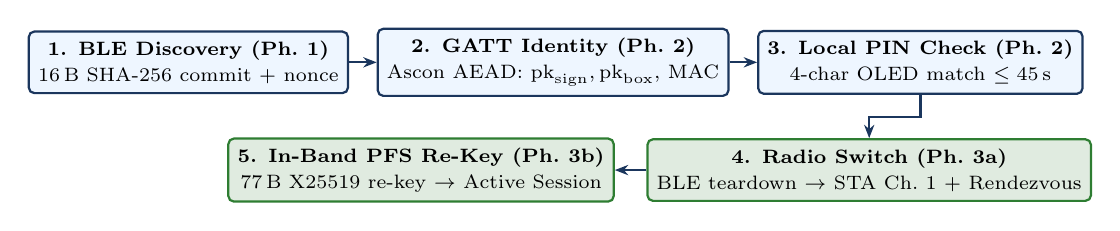
\begin{tikzpicture}[
  node distance=0.45cm and 0.35cm,
  block/.style={rectangle, draw=ieeeBlue, thick, rounded corners=2pt, fill=wsLightBlue, font=\scriptsize, align=center, minimum width=2.40cm, minimum height=0.70cm},
  p3block/.style={rectangle, draw=greenPlot, thick, rounded corners=2pt, fill=greenPlot!15, font=\scriptsize, align=center, minimum width=3.75cm, minimum height=0.70cm},
  arrow/.style={-{Stealth[length=1.7mm,width=1.3mm]}, thick, draw=ieeeBlue}
]
\node[block] (s1) {\textbf{1. BLE Discovery (Ph.\ 1)}\\[1.5pt]16\,B SHA-256 commit + nonce};
\node[block, right=of s1] (s2) {\textbf{2. GATT Identity (Ph.\ 2)}\\[1.5pt]Ascon AEAD: $\text{pk}_{\text{sign}}, \text{pk}_{\text{box}}$, MAC};
\node[block, right=of s2] (s3) {\textbf{3. Local PIN Check (Ph.\ 2)}\\[1.5pt]4-char OLED match $\le 45$\,s};

% Row 2 aligned: s4 under s3/s2, s5 under s2/s1 so both rows span identical width
\node[p3block, below=0.55cm of s3, xshift=-0.65cm] (s4) {\textbf{4. Radio Switch (Ph.\ 3a)}\\[1.5pt]BLE teardown $\rightarrow$ STA Ch.\ 1 + Rendezvous};
\node[p3block, left=0.40cm of s4] (s5) {\textbf{5. In-Band PFS Re-Key (Ph.\ 3b)}\\[1.5pt]77\,B X25519 re-key $\rightarrow$ Active Session};

\draw[arrow] (s1) -- (s2);
\draw[arrow] (s2) -- (s3);
\draw[arrow] (s3.south) -- ++(0,-0.28) -| (s4.north);
\draw[arrow] (s4) -- (s5);
\end{tikzpicture}%
}
\caption{Five-step pairing and handoff sequence: BLE discovery $\rightarrow$ GATT identity exchange $\rightarrow$ local PIN confirmation $\rightarrow$ BLE teardown and Wi-Fi bring-up $\rightarrow$ in-band X25519 PFS re-keying.}
\label{fig:pairing_seq}
\end{figure}

\subsection{Transmit and Receive Paths}
On transmit, \texttt{session\_send\_message()} compresses the message via static Huffman coding and slices it into chunks of $|P_c|\le 58$\,B behind a $2$\,B fragment header (\texttt{[flags|total-1][idx]}). Next, \texttt{stage\_tx\_encrypt} prepares the $24$\,B ESL header to bind it as Ascon-128 associated data, encrypts the $60$\,B payload into $76$\,B, wraps the ciphertext in the outer XSalsa20-HMAC-128 box ($92$\,B), and signs the outer box ciphertext with Ed25519 to emit \texttt{[2B len][92B box][64B sig]} ($158$\,B). Signing the outer ciphertext authenticates the exact wire bytes while binding the ESL header via the inner AEAD tag. In the experimental FEC build, \texttt{stage\_tx\_frame\_fec} appends an inner CRC-32 and encodes Hamming(15,11) ($220$\,B), \texttt{stage\_tx\_esl\_wrap} adds the $24$\,B ESL header and $4$\,B outer CRC ($248$\,B), and \texttt{ecc\_arq\_send()} prepends the $1$\,B ARQ sequence ($249$\,B). In the shipping build (\texttt{CONFIG\_CEEPEW\_FEC\_DISABLE=1}), omitting the $62$\,B FEC expansion yields the $187$\,B wire frame.

On receive, \texttt{process\_rx\_frame()} walks the cost-ordered ingress sequence in Fig.~\ref{fig:receive_path}. Because symmetric tags (outer HMAC-128 and inner Ascon-128 AD tag) are checked before Ed25519 verification, forged frames are rejected in $\approx 1.47$\,ms rather than consuming $663.3$\,ms of curve arithmetic, and the replay bitmap $W$ updates only at Stage~10 after all authenticators pass.

\section{Cryptographic and Framing Protocol Design}

\subsection{Key Schedule, Dual-Layer Cryptographic Analysis, and Ascon-128 v1.2}
The cryptographic stack is listed in Table~\ref{tab:crypto_stack}. Key separation is strictly enforced. CEE-PEW strictly separates the transient Phase~2 GATT bootstrap key (derived strictly from the user code and peer MACs to protect public-key exchange) from the active Phase~3 session keys. For the active session, the user code is expanded into a $32$\,B buffer $c$. A deterministic digit-root preprocessor yields $m = \text{Mix}(c)$, producing the HKDF salt $s = \text{SHA-256}(m \parallel c)$ as a domain-separating pre-whitener (providing salt expansion without claiming additional Shannon entropy). X25519 scalar multiplication computes the master shared secret $K = \text{clamp}(a)\cdot u_m \pmod{2^{255}-19}$, rejecting all seven low-order torsion points in RFC~7748 \S6.1 and any all-zero output. Invalid points are rejected immediately. HKDF-SHA256~\cite{rfc5869} extracts $\text{PRK} = \text{HMAC-SHA256}(s, K)$ and expands domain-separated traffic keys under distinct ASCII info labels: $16$\,B for inner Ascon-128 v1.2 ($K_{\text{ascon}}$), $32$\,B for the outer box ($K_{\text{box}}$), and channel-hopping material ($K_{\text{hop}}$).

\begin{table}[t]
\centering
\caption{Active Cryptographic and Framing Stack}
\label{tab:crypto_stack}
\setlength{\tabcolsep}{3pt}
\scriptsize
\renewcommand{\arraystretch}{0.98}
\begin{tabularx}{\columnwidth}{@{}clXl@{}}
\toprule
\textbf{\#} & \textbf{Primitive / Layer} & \textbf{Protocol Role \& Construction} & \textbf{Implementation} \\
\midrule
1 & X25519 ECDH~\cite{rfc7748} & Ephemeral pairing + PFS re-key & Standalone C (TweetNaCl) \\
2 & Pre-HKDF Mixer & Deterministic 32\,B salt preprocessor (no entropy gain) & Standalone C \\
3 & HKDF-SHA256~\cite{rfc5869} & Domain-separated key schedule & mbedTLS PSA \\
4 & Ascon-128 v1.2~\cite{dobraunig2021} & Inner AEAD ($64$-b rate, $p^{12}/p^6$, +AD) & Standalone C ($19$\,kcycles) \\
5 & XSalsa20 + HMAC-128 & Custom outer EtM cipher + $16$\,B MAC & Standalone C / PSA \\
6 & Ed25519 EdDSA~\cite{bernstein2012} & Per-fragment $64$\,B signature (Full) & Standalone C (TweetNaCl) \\
7 & Nonce Parity + Bitmap & Disjoint 64-b counters ($2^{56}$ cap) & Standalone C \\
\bottomrule
\end{tabularx}
\end{table}

\paragraph{Justification of the Outer XSalsa20-HMAC-128 Layer.} Combining two encryption layers does not automatically strengthen security unless key independence, nonce independence, authentication order, and failure handling are specified:
\begin{enumerate}
\setlength{\itemsep}{0pt}\setlength{\parskip}{0pt}
\item \textit{Exact construction and HMAC subkey derivation:} Our outer layer is \emph{not} a standard Bernstein NaCl \texttt{crypto\_box} (XSalsa20-Poly1305), yet it retains Bernstein's per-packet subkey derivation architecture. Specifically, XSalsa20 consumes the $32$\,B HKDF stream key $K_{\text{box}}$ and the $24$\,B nonce $N$. The first $32$\,B block of the resulting keystream, $K_{\text{mac}}(N) = \text{XSalsa20}_{K_{\text{box}}, N}(0^{32})$, is extracted as a fresh, pseudo-random one-time HMAC key. The outer authenticator is then computed as $T = \text{Trunc}_{128}(\text{HMAC-SHA256}(K_{\text{mac}}(N), C))$, where $C$ is the ciphertext produced by the subsequent keystream block. This guarantees cryptographic key separation between stream cipher and authenticator without requiring an additional HKDF expansion round.
\item \textit{Key and nonce independence:} $K_{\text{ascon}}$ and $K_{\text{box}}$ are derived from HKDF-Expand using disjoint domain-separation labels, making them computationally independent under the PRF assumption on HMAC-SHA256. Nonce collisions are prevented by parity partitioning (even 64-bit counters for initiator, odd for responder, advancing by 2 up to $2^{56}$). From the $24$\,B nonce buffer $\text{session\_id}_{8} \parallel \text{counter}_{8,\text{LE}} \parallel 0_{8}$, Ascon-128 takes the first $16$\,B while XSalsa20 takes all $24$\,B; because the two ciphers are keyed independently and operate on distinct algebraic structures, sharing the 16-byte nonce prefix introduces no cross-primitive related-nonce weakness.
\item \textit{Distinct security properties:} While inner Ascon-128 v1.2 provides AEAD confidentiality and binds the $24$\,B ESL header as Associated Data (AD), the outer XSalsa20-HMAC-128 layer provides (i)~\emph{cryptographic hedge across primitive families} (sponge permutation vs.\ ARX stream cipher + SHA-256 HMAC) and (ii)~\emph{fast outer EtM ingress rejection} ($1.47$\,ms median) before inner decryption or $663.3$\,ms Ed25519 verification. Any failure at either layer triggers identical silent discard (0 feedback bytes), preventing cross-layer oracle leaks. No error codes are returned.
\end{enumerate}

\paragraph{Why Software Ascon-128 v1.2 Over Hardware AES.} Although the ESP32 exposes a hardware AES peripheral ($\approx 10.4$\,MB/s~\cite{oryx_esp32}), software Ascon-128 v1.2 was selected for three reasons. First, software GCM on 32-bit MCUs without \texttt{CLMUL} relies on GF($2^{128}$) tables vulnerable to timing leakage, whereas Ascon's bit-sliced sponge uses only bitwise operations. Second, it avoids FreeRTOS crypto-DMA lock contention across dual cores. Third, protecting a $60$\,B fragment takes $0.12$\,ms ($19$\,kcycles), under $0.5\%$ of a $27$\,ms Lite frame. No hardware coprocessor is assumed. We note that our implementation follows the CAESAR / \textit{J.\ Cryptology} Ascon-128 v1.2 specification ($64$-bit rate, $p^{12}/p^{6}$ rounds)~\cite{dobraunig2021} rather than NIST SP~800-232 \texttt{Ascon-AEAD128} ($128$-bit rate, $p^{12}/p^{8}$ rounds)~\cite{nist_ascon2025}. No SP~800-232 wire interoperability is claimed. Software bit-slicing prevents cache-timing leaks.

\subsection{Verified Wire Frame Budget Across Shipping, Experimental FEC, and Lite Configurations}
Under the ESP-NOW v1.0 ceiling of $250$\,B, compressing each message with static Huffman coding and slicing into chunks of $|P_c| \le 58$\,B yields a closed-form recurrence.
\begin{align}
|F_{\text{in}}| &= |P_c| + 2, \; |C_{\text{ascon}}| = |F_{\text{in}}| + 16, \; |C_{\text{box}}| = |C_{\text{ascon}}| + 16, \label{eq:box}\\
|C_{\text{sig}}| &= |C_{\text{box}}| + 2 + 64 = |P_c| + 100 \le 158\,\text{B}, \label{eq:sig}\\
|C_{\text{fec}}| &= \left\lceil \frac{\lceil 8\,|C_{\text{sig}}| / 11 \rceil \times 15}{8} \right\rceil + 4 \le 220\,\text{B}, \label{eq:fec}\\
|C_{\text{wire,FEC}}| &= |C_{\text{fec}}| + 24_{\text{ESL}} + 4_{\text{CRC}} + 1_{\text{ARQ}} \le 249\,\text{B} \le 250\,\text{B}. \label{eq:wire}
\end{align}
When Hamming(15,11) FEC is compiled out for the shipping Full profile (\texttt{CONFIG\_CEEPEW\_FEC\_DISABLE=1}), the $62$\,B FEC+CRC stage is bypassed ($|C_{\text{wire,ship}}| = |C_{\text{sig}}| + 24_{\text{ESL}} + 4_{\text{CRC}} + 1_{\text{ARQ}} = 187$\,B). Table~\ref{tab:frame_budget} and Fig.~\ref{fig:wire_budget} present the exact byte breakdown across all configurations.

\begin{table}[t]
\centering
\caption{Wire Frame Budget for a $58$\,B Chunk Across Shipping Full (No FEC), Experimental Full (With FEC), and Lite Profiles}
\label{tab:frame_budget}
\setlength{\tabcolsep}{2.2pt}
\scriptsize
\renewcommand{\arraystretch}{0.98}
\begin{tabularx}{\columnwidth}{@{}>{\raggedright\arraybackslash}p{0.18\columnwidth}>{\raggedright\arraybackslash}Xrrrr@{}}
\toprule
\textbf{Stage} & \textbf{Transformation} & \textbf{Delta} & \textbf{Ship Full} & \textbf{Exp.\ FEC} & \textbf{Ship Lite} \\
\midrule
1. Huffman Slice & Chunk ($|P_c|$) & --- & $58$\,B & $58$\,B & $58$\,B \\
2. Frag Header & \texttt{[flags|tot][idx]} & $+2$\,B & $60$\,B & $60$\,B & $60$\,B \\
3. Inner AEAD & Ascon-128 + $16$\,B tag & $+16$\,B & $76$\,B & $76$\,B & $76$\,B \\
4. Outer Box & XSalsa20 + HMAC-128 & $+16$\,B & $92$\,B & $92$\,B & \textit{Omitted} \\
5. Sign \& Prefix & \texttt{uint16} + Ed25519 sig & $+66$\,B & $158$\,B & $158$\,B & \textit{Omitted} \\
6. Permuted FEC & Hamming(15,11) + CRC & $+0$/$62$\,B & \textit{Disabled} & $220$\,B & \textit{Disabled} \\
7. ESL Framing & $24$\,B ESL + outer CRC & $+28$\,B & $186$\,B & $248$\,B & $104$\,B \\
8. Retry Byte & MAC-ACK ARQ seq & $+1$\,B & $\mathbf{187\,\textbf{B}}$ & $\mathbf{249\,\textbf{B}}$ & $\mathbf{105\,\textbf{B}}$ \\
\midrule
\multicolumn{6}{@{}>{\raggedright\arraybackslash}p{\dimexpr\columnwidth-1pt}@{}}{\textit{Payload efficiency at $|P_c|=58$\,B:} Shipping Full $\mathbf{31.0\%}$ ($187$\,B); Experimental Full w/ FEC $\mathbf{23.3\%}$ ($249$\,B); Shipping Lite no FEC $\mathbf{55.2\%}$ ($105$\,B); Lite w/ FEC $\mathbf{42.0\%}$ ($138$\,B). \textit{Max chunk $|P_c|$ in $249$\,B v1.0 (w/ FEC / no FEC):} Full $58$\,B / $120$\,B; Lite $140$\,B / $202$\,B. \textit{ESP-NOW v2.0 ($1{,}470$\,B, amortized estimate only):} Full $953$/$1{,}341$\,B; Lite $1{,}035$/$1{,}423$\,B.} \\
\bottomrule
\end{tabularx}
\end{table}

\begin{figure}[t]
\centering
\resizebox{\columnwidth}{!}{%
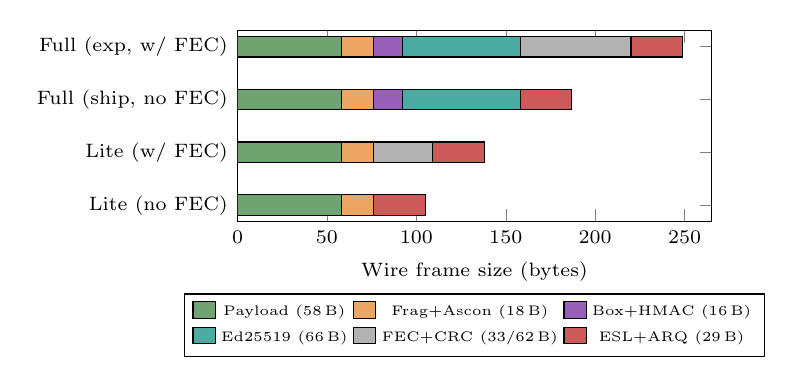
\begin{tikzpicture}
\begin{axis}[
    width=7.6cm,
    height=4.0cm,
    xbar stacked,
    bar width=7.5pt,
    xlabel={Wire frame size (bytes)},
    xlabel style={font=\scriptsize},
    symbolic y coords={{Lite (no FEC)}, {Lite (w/ FEC)}, {Full (ship, no FEC)}, {Full (exp, w/ FEC)}},
    ytick=data,
    y tick label style={font=\scriptsize},
    x tick label style={font=\scriptsize},
    legend style={at={(0.5,-0.38)},anchor=north,legend columns=3,font=\tiny},
    xmin=0,
    xmax=265,
]
\addplot[fill=greenPlot!70] coordinates {(58,{Lite (no FEC)}) (58,{Lite (w/ FEC)}) (58,{Full (ship, no FEC)}) (58,{Full (exp, w/ FEC)})};
\addplot[fill=orangePlot!70] coordinates {(18,{Lite (no FEC)}) (18,{Lite (w/ FEC)}) (18,{Full (ship, no FEC)}) (18,{Full (exp, w/ FEC)})};
\addplot[fill=purplePlot!70] coordinates {(0,{Lite (no FEC)}) (0,{Lite (w/ FEC)}) (16,{Full (ship, no FEC)}) (16,{Full (exp, w/ FEC)})};
\addplot[fill=tealPlot!70] coordinates {(0,{Lite (no FEC)}) (0,{Lite (w/ FEC)}) (66,{Full (ship, no FEC)}) (66,{Full (exp, w/ FEC)})};
\addplot[fill=gray!60] coordinates {(0,{Lite (no FEC)}) (33,{Lite (w/ FEC)}) (0,{Full (ship, no FEC)}) (62,{Full (exp, w/ FEC)})};
\addplot[fill=wsRed!70] coordinates {(29,{Lite (no FEC)}) (29,{Lite (w/ FEC)}) (29,{Full (ship, no FEC)}) (29,{Full (exp, w/ FEC)})};
\legend{Payload ($58$\,B), Frag+Ascon ($18$\,B), Box+HMAC ($16$\,B), Ed25519 ($66$\,B), FEC+CRC ($33$/$62$\,B), ESL+ARQ ($29$\,B)}
\end{axis}
\end{tikzpicture}%
}
\caption{Wire budget breakdown for $P_c{=}58$\,B across all four configurations: Shipping Lite (105\,B), Experimental Lite w/ FEC (138\,B), Shipping Full (187\,B), and Experimental Full w/ FEC (249\,B).}
\label{fig:wire_budget}
\end{figure}

\begin{figure*}[t]
\centering
\includegraphics[width=\textwidth]{ceepew_wireshark_real_crop.pdf}
\caption{Wireshark GUI captures of the CEE-PEW over-the-air runs with the released Lua dissector loaded (unedited screen captures): (a) Mode~B, standard 802.11 CCMP Action frames between the two device MACs (\texttt{wlan.addr} filter); (b) Mode~C, CEE-PEW Extended Security Layer (ESL) frames selected by \texttt{ceepew.esl.magic0} and decoded into per-frame \texttt{seq}/\texttt{nonce} columns. The two panels come from separate capture runs on Channel~1.}
\label{fig:wireshark_real}
\end{figure*}

\section{Reliability Engineering and Cost-Ordered RX}

\subsection{Session-Permuted Hamming(15,11) FEC Ablation vs.\ IEEE 802.11 FCS}
In the experimental FEC build, the $158$\,B signed block is cut into 11-bit slices, encoded into 15-bit Hamming(15,11) codewords~\cite{hamming1950} ($\eta = 4/11 \approx 36.4\%$ parity overhead~\cite{lin2004}), and permuted via a session-keyed Fisher-Yates shuffle. Because Hamming(15,11) is a single-error-correcting (SEC) code rather than SECDED, double-bit errors may be mis-corrected by the 16-entry syndrome table and are caught downstream by the inner CRC-32 and AEAD tags.

Standard IEEE 802.11 receivers validate the 32-bit MAC Frame Check Sequence (FCS) in hardware and drop corrupted frames before invoking the ESP-NOW callback~\cite{yin2020}. In Campaign X6 (\texttt{data/raw/X6\_fec\_ablation\_20261030/}), two sealed builds differing only by \texttt{CONFIG\_CEEPEW\_FEC\_DISABLE} were tested over our $\approx 1$\,m LOS indoor link. Both configurations were tested thoroughly. FEC-ON ($249$\,B wire frame) delivered 50/53 messages (94.3\%) in 499.5\,s; FEC-OFF ($187$\,B shipping frame) delivered 45/48 (93.8\%) in 600\,s. Across $97$--$99$ RX fragments per arm, \textbf{zero single-bit errors were corrected in either arm}. Hardware FCS drops corrupt frames first. We qualify this negative finding carefully: it establishes that software FEC provided no measurable benefit over standard non-promiscuous ESP-NOW callbacks under clean, short-range LOS conditions where the 802.11 FCS filters corrupted MPDUs first. It does \emph{not} establish that FEC is universally unnecessary for ESP-NOW; FEC may still provide coding gain when promiscuous FCS-fail reception (\texttt{WIFI\_PROMISCUOUS\_FILTER\_MASK\_FCSFAIL})~\cite{yin2020} is enabled or under harsh interference/multipath regimes.

\subsection{Delivery Semantics, Sliding-Bitmap Replay Window, and Channel-Hopping Discrepancy}
\paragraph{Correction of Delivery Semantics.} We explicitly distinguish MAC-layer acknowledgement from application-layer delivery. Specifically, \textbf{CEE-PEW provides MAC-acknowledged transmission with receiver-side duplicate suppression and no application-layer delivery guarantee.} Sender retransmission is driven by the ESP-NOW send callback (up to 5 attempts---initial + 4 retries---with a $600$\,ms timeout and jittered exponential backoff $b(n) = 100\cdot 2^{\min(n,2)}\cdot(1+\varepsilon)$\,ms, bounding worst-case per-fragment retry at $\approx 4{,}100$\,ms). The receiver's 802.11 hardware emits the $14$\,B MAC ACK (Frame Control field \texttt{0x00D4} (transmitted as \texttt{0xD4} \texttt{0x00}, Type \texttt{01b} Control, Subtype \texttt{1101b} ACK)) immediately upon valid physical FCS reception---\emph{before} the frame enters \texttt{g\_session\_rx\_queue} or undergoes cryptographic verification. Consequently, a fragment whose MAC ACK succeeded is still silently dropped without sender retransmission if the 32-deep RX queue overflows during slow $663.3$\,ms verification, if authentication fails, or if the static region extent table fills during multi-fragment reassembly. Without an application-level ACK/NACK mechanism (reserved for future work), a single lost fragment invalidates a multi-fragment message without sender notification. Accordingly, we separate five distinct metrics: (1)~fragment MAC transmission success, (2)~RX queue ingress, (3)~fragment authentication \& replay commit, (4)~complete message reassembly, and (5)~application-level confirmation.

\paragraph{Session Identifier Generation and Nonce Lifecycle.} Nonce uniqueness across power cycles and re-key events is strictly enforced. The 8-byte session identifier $\text{session\_id}_8$ is drawn directly from the ESP32 hardware True Random Number Generator (CSPRNG via \texttt{bootloader\_random()}/\texttt{esp\_fill\_random()}) upon each pairing negotiation and refreshed on every in-band X25519 PFS re-key. Nonce counters reset to their role-determined initial values (0 for initiator, 1 for responder) only when a fresh $\text{session\_id}_8$ and rotated traffic keys are committed. All session parameters and counters reside exclusively in volatile internal SRAM. Upon reboot or watchdog reset, \texttt{crypto\_ctx\_destroy()} securely zeroizes all key material and counters, requiring nodes to re-pair before transmitting application frames. Counter wraparound is prohibited: counters are strictly bounded at $2^{56}$, and nodes transition to \texttt{FAILED} if the bound is reached without prior re-keying.

\paragraph{Session Identifier Generation and Nonce Lifecycle.} Nonce uniqueness across power cycles and re-key events is strictly enforced. The 8-byte session identifier $\text{session\_id}_8$ is drawn directly from the ESP32 hardware True Random Number Generator (CSPRNG via \texttt{bootloader\_random()}/\texttt{esp\_fill\_random()}) upon each pairing negotiation and refreshed on every in-band X25519 PFS re-key. Nonce counters reset to their role-determined initial values (0 for initiator, 1 for responder) only when a fresh $\text{session\_id}_8$ and rotated traffic keys are committed. All session parameters and counters reside exclusively in volatile internal SRAM. Upon reboot or watchdog reset, \texttt{crypto\_ctx\_destroy()} securely zeroizes all key material and counters, requiring nodes to re-pair before transmitting application frames. Counter wraparound is prohibited: counters are strictly bounded at $2^{56}$, and nodes transition to \texttt{FAILED} if the bound is reached without prior re-keying.

\paragraph{Sliding-Bitmap Replay Window.} The ESL ingress path executes in bounded order before curve arithmetic.
\begin{equation}
\text{\footnotesize DoS}\!\rightarrow\!\text{\footnotesize MAC}\!\rightarrow\!\text{\footnotesize Magic}\!\rightarrow\!\text{\footnotesize CRC}\!\rightarrow\!\text{\footnotesize Time}\!\rightarrow\!\text{\footnotesize Replay}\!\rightarrow\!\text{\footnotesize FEC/AEAD}.
\label{eq:rx_order}
\end{equation}
The Replay stage maintains a 64-bit sliding bitmap~\cite{donenfeld2017} $W$ anchored to the highest authenticated sequence $s_{\max}$, admitting sequence $s$ if and only if:
\begin{equation}
s > s_{\max} \quad \lor \quad \left(s_{\max} - s < 64 \;\land\; W[s_{\max} - s] = 0\right).
\label{eq:replay}
\end{equation}
Because the $24$\,B ESL header is bound as Ascon-128 associated data and $W$ commits only after both the AD-bound tag and Ed25519 signature pass, forged or header-edited frames never advance $s_{\max}$ or evict valid window slots. Replay updates follow authentication strictly.

\paragraph{Channel-Hopping Evidence Separation.} We separate four distinct levels of evidence for nine-channel frequency hopping. First, regarding \textit{algorithm design}, a counter-indexed Fisher-Yates permutation $p$ of $\{1,\dots,9\}$ updates every \texttt{CEEPEW\_HOP\_INTERVAL\_MS} $= 5{,}000$\,ms. Second, regarding the \textit{disclosed implementation defect}, setting $n = e \wedge \neg 1$, $k = (n \gg 6) \bmod 256$, and indexing $p[(n \gg 14) \bmod 9]$ leaves the index at $0$ for the first $16{,}384$ epochs. In that state, the permutation seed $k$ advances only once per $64$ epochs ($320$\,s realized dwell instead of $5$\,s). Third, \textit{functionality} remains unverified over the air. Fourth, \textit{performance} was not measured, as hopping was disabled (\texttt{CONFIG\_CEEPEW\_CHANNEL\_HOP=0}) across all evaluated empirical builds. Hopping was omitted during testing.

\section{Implementation Challenges, Ed25519 Bottleneck Isolation, and Verification Cache}

\paragraph{Sequential Radio Teardown Ordering.} Early teardown code deinitialized Bluedroid while the BLE controller remained active, causing an in-flight HCI command-complete event to race into a freed mutex. The resolved sequence closes the GATT link, drains the event queue ($200$\,ms), disables Bluedroid (awaiting HCI reset), disables the BLE controller, waits $50$\,ms, deinitializes host and controller, and waits $250$\,ms before initializing Wi-Fi STA.

\paragraph{Isolating the $663.3$\,ms Ed25519 Bottleneck (TweetNaCl Port vs.\ ESP32 Hardware).}\label{sec:vc} To establish whether our $663.281$\,ms Ed25519 verification latency is an architectural limitation of the ESP32 or an implementation artifact, we document five exact parameters. First, our \textit{TweetNaCl source} is a standalone C port of public-domain \texttt{tweetnacl.c} (20140427 release) with an unwindowed 255-step scalar ladder, saving $32$\,KB of flash over unrolled \texttt{ref10}. Second, the \textit{compiler} is \texttt{xtensa-esp32-elf-gcc} (ESP-IDF v6.0.3) built at \texttt{-O2} in Campaign X1 (vs.\ \texttt{-Og} in the $1{,}075$\,ms unoptimised baseline) at a fixed $160$\,MHz clock. Third, regarding \textit{64-bit vs.\ 32-bit limb arithmetic}, TweetNaCl stores $\text{GF}(2^{255}-19)$ elements as sixteen signed 64-bit limbs (\texttt{int64\_t gf[16]}), forcing the 32-bit Xtensa LX6 core to emulate $64\times 64$-bit multiplications and carry propagation in software across 255 iterations. Fourth, the \textit{stack footprint} consumes $<2.4$\,KB of stack on Core~1's $16{,}384$\,B stack, with $0$\,B of heap. Fifth, under \textit{clock-normalized comparison}, 32-bit radix-$2^{25.5}$ implementations on the ESP32 (CycloneCRYPTO at \texttt{-O3}~\cite{oryx_esp32}) require $3.9$\,Mcycles for X25519 and $6.8$\,Mcycles for Ed25519 verify---equivalent to $\mathbf{24.4\,\textbf{ms}}$ and $\mathbf{42.5\,\textbf{ms}}$ at $160$\,MHz ($15.6\times$ faster than our $663.3$\,ms port). This confirms that the bottleneck is implementation-specific rather than architectural. The delay stems from limb emulation.

\paragraph{Duplicate Verification and Proposed Verification Cache.} Because the $600$\,ms sender ARQ timeout is shorter than the $663.3$\,ms verification time, a retransmitted duplicate arrives before the original commits at Stage~10, passes the read-only replay check, and incurs a second $663.3$\,ms verification (halving goodput from $74$--$88$\,B/s to $44$\,B/s). Likewise, back-to-back $365.5$\,ms sends overflow the 32-deep RX queue after $\approx 71$ fragments. Elevating our proposed \textbf{Verification Cache}, we specify a 4-slot table preceding Stage~7 keyed by \texttt{(session\_id, esl\_seq, sha256\_frame\_digest[0..15])}. Caching the 16-byte SHA-256 digest of a verified wire frame allows byte-identical retransmissions to bypass curve arithmetic (dropping duplicate processing from $727.3$\,ms to $\approx 63$\,ms) The proposed cache binds duplicate suppression to the session identifier, sequence number, and a truncated 16-byte cryptographic frame digest, preventing straightforward sequence-number-only substitution. Cache invalidation is tied to PFS re-keying and replay-window advancement. We note that this Verification Cache represents an unmeasured proposed architecture reserved for future firmware revisions.

\section{Testing Methodology and Experimental Setup}

\subsection{Test-Bed Topology, Shared Sync Wire (\texttt{GPIO14}), and Third-Board Sniffer}\label{sec:hop-disabled}\label{sec:sniffer}\label{sec:capture}
The test bed comprises two ESP32 DevKit~v1 boards placed $20$\,cm apart on Channel~1 (hopping disabled) and a third independent ESP32 running promiscuous sniffer firmware (\texttt{components/sniffer/}, filtering OUI \texttt{18:fe:34} and streaming hex frames over UART1 at $921{,}600$\,baud to \texttt{serial\_to\_pcap.py}). Because independent \texttt{esp\_timer} clocks never synchronize, an open-drain jumper on \texttt{GPIO14} links the pair. Immediately before radio submission, the transmitter drives \texttt{GPIO14} LOW, and both boards timestamp the falling edge against their own local crystal. Thus all four reported intervals---TX $\text{submit}\rightarrow\text{pulse}$ and $\text{pulse}\rightarrow\text{send\_cb}$, and RX $\text{edge}\rightarrow\text{rx\_cb}$ and $\text{rx\_cb}\rightarrow\text{accept}$---difference two readings from the \emph{same} board clock.

Timing sessions run completely silent (no UART logging inside measured regions) and seal raw logs under SHA-256 manifests (Campaign X1, commit \texttt{b263dde-dirty}, ESP-IDF v6.0.3). Confidence intervals are computed via $10{,}000$-draw cluster bootstrapping~\cite{efron1979bootstrap} over board--iteration pairs in \texttt{stats\_core.py}. On the host tier, $17$ test suites compiled under ASan and UBSan verify RFC~8032, RFC~7748, RFC~5869, and Ascon-128 v1.2 vectors alongside a $100$-vector replay injection campaign.

\section{Threat Model and Disclosed Limitations}
Table~\ref{tab:threat} summarizes the audited threat model and disclosed limitations. Five protocol and implementation risks warrant explicit disclosure:
\begin{itemize}
\setlength{\itemsep}{0pt}\setlength{\parskip}{0pt}
\item \textbf{Experimental 4-Character Pairing Protocol (Distinguishing Three Security Properties):} The user selects a $4$-character code from a $36$-symbol alphabet ($36^4 = 1{,}679{,}616$ combinations; $1{,}679{,}615$ usable). Each node computes the commitment $C = \text{SHA-256}(\texttt{CEEPEW\_COMMIT\_v2} \parallel \mathit{id}_A \parallel \mathit{id}_B \parallel \text{code}_{32} \parallel t_{\mathrm{round}})$ with $t_{\mathrm{round}}=0$, transmitting its first $16$\,B in the BLE discovery beacon and all $32$\,B over GATT. We explicitly distinguish three security properties for the pairing design. First, \emph{code matching and transcript consistency} is provided: mismatched user codes produce commitment mismatches that abort pairing fail-closed. Second, \emph{resistance to offline password guessing} is not provided: because $\mathit{id}_A$, $\mathit{id}_B$, $t_{\mathrm{round}}=0$, and $C$ travel over the air, an eavesdropper capturing $C$ can enumerate all $1.68\text{M}$ candidate codes offline and recover the GATT identity key. Third, \emph{authentication against an active MITM} is not provided: this commitment scheme is not a Password-Authenticated Key Exchange (PAKE), and displaying matching codes does not stop an active MITM during the $45$\,s window from substituting its own keys. Migration to SPAKE2+~\cite{rfc9383} and Tamarin verification~\cite{vanderlinden2023} are planned to close this gap~\cite{vontschirschnitz2021,jangid2023}.
\item \textbf{Xtensa Compiler Timing Leaks (CVE-2025-12888):} While our TweetNaCl X25519 ladder uses branchless C swaps and passes a host Welch's $t$-test ($|t|<4.5$), CVE-2025-12888~\cite{cve2025_12888} demonstrates that \texttt{xtensa-esp32-elf-gcc} can emit secret-dependent branches from branchless source. Side-channel resistance is therefore claimed at the source level only (\textit{Partial}).
\item \textbf{OUI and Cleartext ESL Header Fingerprinting:} Wireless IDS sensors can fingerprint Espressif's OUI~\cite{guardianair2024} and the cleartext $24$\,B ESL header (\texttt{0x4553} magic, monotonic \texttt{seq}/\texttt{nonce\_counter}).
\item \textbf{Physical SRAM Exposure:} Session keys reside in SRAM (zeroed at teardown via \texttt{ceepew\_secure\_zero()}) without secure enclave binding, and the $48$\,KB \texttt{.bss} pool sits outside flash encryption.
\item \textbf{Residual BLE Context-Mutex Defect in Evaluated Build (\texttt{b263dde-dirty}):} \texttt{BUG-BLE-CTX-LOCK-PANIC}, an intermittent BLE context-mutex panic on entry to \texttt{IDLE} before the post-derive barrier, remains present in the evaluated firmware binary (\texttt{b263dde-dirty}) used for Campaigns X1--X12. The candidate patch (\texttt{FIX-BLE-CTX-RELEASE}) is compile-verified only and was not flashed into the evaluated binaries prior to a $5$\,h hardware regression run.
\end{itemize}

\begin{table}[t]
\caption{Audited Threat Coverage and Disclosed Limitations}
\label{tab:threat}
\centering\scriptsize
\setlength{\tabcolsep}{2.5pt}
\renewcommand{\arraystretch}{1.05}
\begin{tabularx}{\columnwidth}{@{}>{\raggedright\arraybackslash}p{0.23\columnwidth}>{\raggedright\arraybackslash}p{0.18\columnwidth}>{\raggedright\arraybackslash}X@{}}
\toprule
\textbf{Threat Vector} & \textbf{Status} & \textbf{Mechanism / Disclosed Limitation}\\
\midrule
Cleartext injection \& OOB DoS & Mitigated (design + host) & Mandatory ESL with AD-bound Ascon-128 tag and static bounds mitigates Issue \#15179~\cite{espressif_issue15179}; unaffected by middleware CVE-2024-42484~\cite{nozomi2024}.\\
Offline guessing \& active MITM on 4-char pairing code & \textbf{Disclosed (Experimental)} & Commitment $C$ over $36^4$ codes confirms transcript match but is vulnerable to offline dictionary enumeration and active MITM identity substitution; SPAKE2+~\cite{rfc9383} required.\\
DoS / CPU amplification (forged fresh seq) & Partially mitigated & Cost-ordered RX rejects forged frames at outer Box HMAC in $1.29$\,ms median ($N=10$; $\approx 10.3$\,ms total RX cost), avoiding $663.3$\,ms Ed25519; $\approx 100$ forged frames/s saturate Core~1.\\
Cache-eviction replay (CVE-2024-42483) & Mitigated (host verified) & Disjoint 64-b parity nonces + 64-b sliding bitmap $W$ committed post-auth. 100/100 replay and 24/24 header-tamper vectors rejected on host harness (no OTA RF replay test).\\
Multi-fragment region exhaustion & Disclosed limit & Sustained incompressible multi-fragment bursts can exhaust the 256-entry region table (\texttt{err=9}) after MAC ACK; single frames ($\le 249$\,B) unaffected.\\
Side channel (CVE-2025-12888) & Partial (source only) & Branchless C X25519 passes host Welch $t$-test ($|t|<4.5$), but Xtensa GCC may emit non-constant-time machine code~\cite{cve2025_12888}.\\
Residual BLE mutex defect & \textbf{Disclosed (\texttt{b263dde})} & \texttt{BUG-BLE-CTX-LOCK-PANIC} present in evaluated binary; patch \texttt{FIX-BLE-CTX-RELEASE} is compile-verified but not flashed in reported runs.\\
\bottomrule
\end{tabularx}
\end{table}

\section{Empirical Evaluation and Hardware Profiling}\label{sec:evaluation}

\begin{figure*}[t]
\centering
\includegraphics[width=\textwidth]{ceepew_verified_panels.pdf}
\caption{Measured behaviour of the two-node test bed. (a) Per-stage execution latency, minimum to maximum with the median marked, on a logarithmic axis ($N=98$--$114$). (b) 802.11 MPDU lengths of the $90$ captured CEE-PEW frames on Channel~1, where the $217$\,B mode is the data frame. (c) Secondary sanity check showing pooled-byte Shannon entropy over the byte counts shown (Mode-A plaintext $6.79$ vs.\ CEE-PEW ESL body $7.34$\,bits/byte).}
\label{fig:verified_panels}
\end{figure*}

\subsection{Ascon-128 v1.2 KAT, Lua Dissector, and Replay Suite}
Standalone C primitives were verified byte-exactly against RFC~8032 Ed25519, RFC~7748 X25519, RFC~5869 HKDF-SHA256, and the official Ascon-128 v1.2 reference vectors~\cite{dobraunig2021} on both the host ASan/UBSan harness and the on-device boot KAT (Table~\ref{tab:hex_comparison}). Over-the-air ESL frames were decoded using our released Wireshark Lua post-dissector (\path{ceepew_wireshark_dissector.lua}, Fig.~\ref{fig:wireshark_real}).

\begin{table}[t]
\centering
\caption{Ascon-128 v1.2 Reference Vectors (Part A) and Protocol Security Comparison (Part B)}
\label{tab:hex_comparison}
\setlength{\tabcolsep}{2.5pt}
\scriptsize
\renewcommand{\arraystretch}{0.98}
\begin{tabularx}{\columnwidth}{@{}>{\raggedright\arraybackslash}p{0.28\columnwidth}>{\raggedright\arraybackslash}p{0.18\columnwidth}>{\raggedright\arraybackslash}p{0.19\columnwidth}>{\raggedright\arraybackslash}X@{}}
\toprule
\multicolumn{4}{@{}>{\raggedright\arraybackslash}p{\dimexpr\columnwidth-1pt}@{}}{\textbf{Part A: Ascon-128 v1.2 AEAD KAT.} \texttt{Key=0001..0f}, \texttt{Nonce=0001..0f}, \texttt{AD=00010203}, \texttt{PT=0001020304050607}; expected $8$\,B CT $\parallel$ $16$\,B tag: {\tiny\texttt{7763f8ba6ce91ed1 c2e6d6fa2309ef26 d1e6df20faeb33a6}} --- \textbf{100\% Match (Host \& ESP32 Boot KAT)}~\cite{dobraunig2021}.} \\
\midrule
\textbf{Property} & \textbf{Core CCMP} & \textbf{\texttt{esp-now} ($<$2.5.2)} & \textbf{CEE-PEW (Lite / Ship Full)} \\
\midrule
$58$\,B chunk wire / $1$\,Mbps airtime & $74$\,B / $1.13$\,ms~\cite{espressif_espnow} & $\approx 86$\,B / $1.22$\,ms~\cite{nozomi2024} & $\mathbf{105}$\,\textbf{B} ($1.376$\,ms) / $\mathbf{187}$\,\textbf{B} ($2.032$\,ms), computed \\
Unencrypted RX injection~\cite{espressif_issue15179} & \textbf{Accepted (vuln.)} & App-filtered & \textbf{Rejected} ($0$\,B feedback; host fault-injection) \\
$100$-vector host replay ($4\times 25$): & & & \\
\quad Recent dup.\ ($0 \le \Delta < 25$) & No cache & Rejected~\cite{nozomi2024} & \textbf{Rejected ($25/25$)} \\
\quad Mid-window ($25 \le \Delta < 50$) & No cache & Rejected~\cite{nozomi2024} & \textbf{Rejected ($25/25$)} \\
\quad Stale ($s \le s_{\max}-64$) & Accepted~\cite{nozomi2024} & \textbf{Accepted ($>32$ fr.)} & \textbf{Rejected ($25/25$)} \\
\quad CVE-2024-42483 eviction & Accepted~\cite{nozomi2024} & \textbf{Accepted (vuln.)} & \textbf{Rejected ($25/25$)} \\
ESL AD header tamper ($24$ vec.) & N/A & Unauthenticated & \textbf{Rejected ($24/24$)} \\
\bottomrule
\end{tabularx}
\end{table}

\subsection{Split Hardware Profiling: Stage Execution Latencies (Table VI) and Airtime/Reliability Metrics (Table VII)}
To ensure clarity, we separate per-stage MCU execution timings (Table~\ref{tab:hw_benchmarks} and Fig.~\ref{fig:stage_timing}) from end-to-end sync-wire intervals, multi-stage delivery accounting, and memory usage (Table~\ref{tab:reliability_mem}). Across two bidirectional runs in Campaign X8 (Table~\ref{tab:reliability_mem}), MAC-layer send callbacks reported $100\%$ completion ($38/38$ and $36/36$), whereas application-layer Huffman decompression confirmation reached $92.1\%$ ($35/38$) and $91.7\%$ ($33/36$)---an $\approx 8$\,pp gap caused by post-MAC-ACK ESL discards (\texttt{err=3}) and ARQ decode drops (\texttt{err=17}).

\begin{table}[t]
\centering
\caption{ESP32 Per-Stage Cryptographic Execution Latencies at $160$\,MHz}
\label{tab:hw_benchmarks}
\setlength{\tabcolsep}{2.5pt}
\scriptsize
\renewcommand{\arraystretch}{0.98}
\begin{tabularx}{\columnwidth}{@{}>{\raggedright\arraybackslash}p{0.36\columnwidth}r>{\raggedright\arraybackslash}X@{}}
\toprule
\textbf{Cryptographic / Framing Stage} & \textbf{Cycles} & \textbf{ESP32 Time (Med., IQR, 95\%\,CI)} \\
\midrule
\multicolumn{3}{@{}l@{}}{\textbf{Handshake \& In-Band PFS Re-Key (Wall-Clock)}} \\
\quad Clean BLE pairing $\rightarrow$ ESP-NOW handoff & $1{,}037$\,Mcycles & $6.48$\,s ($3.22$\,s GATT, \texttt{-Og}) \\
\quad In-band ESP-NOW PFS X25519 re-key ($77$\,B) & --- & $4.09$--$4.47$\,s (wall-clock, \texttt{-O2}) \\
\midrule
\multicolumn{3}{@{}l@{}}{\textbf{Symmetric \& Framing Stages ($58$\,B Chunk)}} \\
\quad Static Huffman compress / decompress & $0.13\text{--}0.47$\,M & $1.0$\,ms med.\ ($3$\,ms @ $132$\,B) \\
\quad TX Inner Ascon-128 v1.2 ($60\,\text{B}\rightarrow 76\,\text{B}$) & $\mathbf{0.019}$\,\textbf{M} & $\mathbf{0.12}$\,\textbf{ms} ($123\,\mu$s profiled, X12) \\
\quad RX Inner Ascon-128 decrypt (\texttt{-O2}) & $0.053$\,M & $\mathbf{0.33}$\,\textbf{ms} (IQR $0.09$, CI $[0.31,0.40]$; $N{=}97$) \\
\quad RX Outer Box decrypt (XSalsa20+HMAC, \texttt{-O2}) & $0.235$\,M & $\mathbf{1.47}$\,\textbf{ms} (IQR $0.23$, CI $[1.33,1.55]$; $N{=}98$) \\
\quad RX Forged-frame outer Box reject (X5, \texttt{-O2}) & $0.206$\,M & $\mathbf{1.29}$\,\textbf{ms} (IQR $0.17$, CI $[1.24,1.41]$; $N{=}10$) \\
\quad Permuted Hamming(15,11) + inner CRC (TX) & $0.48$\,M & $3.0$\,ms (IQR $1.0$, range $2\text{--}5$\,ms) \\
\quad ESL wrap (TX) / 10-stage unwrap (RX) & $1.12$/$1.44$\,M & $7.0$\,ms TX / $9.0$\,ms RX (IQR $2.0$) \\
\midrule
\multicolumn{3}{@{}l@{}}{\textbf{Asymmetric Curve Stages (64-b Limb TweetNaCl vs.\ 32-b Reference)}} \\
\quad \textbf{X25519 Scalar Mult.} (Campaign X1, \texttt{-O2}) & $23.67$\,M & $\mathbf{147.957}$\,\textbf{ms} (CI $[147.925,148.002]$; $N{=}50$) \\
\quad \textbf{Ed25519 Sign} (Campaign X1, \texttt{-O2}) & $53.16$\,M & $\mathbf{332.257}$\,\textbf{ms} (CI $[332.222,332.349]$; $N{=}49$) \\
\quad \textbf{Ed25519 Verify} (Campaign X1, \texttt{-O2}) & $106.12$\,M & $\mathbf{663.281}$\,\textbf{ms} (CI $[663.200,663.332]$; $N{=}50$) \\
\quad Uncached Box / Ed25519 (\texttt{-Og} baseline) & $35.0$/$172.0$\,M & $219.0$\,ms (Box) / $1{,}075.0$\,ms (Ed25519) \\
\quad \textit{Ref.: 32-b radix-$2^{25.5}$ @ \texttt{-O3} (scaled to $160$\,MHz)~\cite{oryx_esp32}} & \textit{$3.9$/$6.8$\,M} & \textit{$\mathbf{24.4}$\,\textbf{ms} (X25519) / $\mathbf{42.5}$\,\textbf{ms} (Verify)} \\
\bottomrule
\end{tabularx}
\end{table}

\begin{table}[t]
\centering
\caption{Physical Airtime, Sync-Wire Intervals, Delivery Accounting, and Memory Footprint}
\label{tab:reliability_mem}
\setlength{\tabcolsep}{2.5pt}
\scriptsize
\renewcommand{\arraystretch}{0.98}
\begin{tabularx}{\columnwidth}{@{}>{\raggedright\arraybackslash}p{0.38\columnwidth}>{\raggedright\arraybackslash}X@{}}
\toprule
\textbf{Metric / Interval} & \textbf{Measured Hardware Value / Distribution} \\
\midrule
\multicolumn{2}{@{}l@{}}{\textbf{Airtime \& Same-Clock Sync-Wire (\texttt{GPIO14}) Intervals ($N=80$ TX, $N=71/68$ RX)}} \\
\quad $1$\,Mbps physical airtime (computed) & $\mathbf{2.032}$\,\textbf{ms} ($187$\,B ship) / $\mathbf{2.528}$\,\textbf{ms} ($249$\,B FEC; $2.84$\,ms w/ ACK) \\
\quad ESP-NOW send-callback latency ($N{=}76$) & $\mathbf{18.0}$\,\textbf{ms} med.\ (IQR $2.25$\,ms; includes $\approx 15.5$\,ms OS/driver overhead) \\
\quad TX $\text{submit}\rightarrow\text{pulse}$ (Full, \texttt{-O2}) & $\mathbf{365.5}$\,\textbf{ms} Dev A (IQR $357.3$--$371.7$) / $\mathbf{370.3}$\,\textbf{ms} Dev B \\
\quad TX $\text{pulse}\rightarrow\text{send\_cb}$ (Full, \texttt{-O2}) & $\mathbf{4.36}$\,\textbf{ms} Dev A (IQR $4.22$--$4.63$) / $\mathbf{4.36}$\,\textbf{ms} Dev B \\
\quad RX $\text{edge}\rightarrow\text{rx\_cb}$ (One-Way Driver+Air) & $\mathbf{26.6}$\,\textbf{ms} Dev A (IQR $20.1$--$37.6$) / $\mathbf{27.2}$\,\textbf{ms} Dev B \\
\quad RX $\text{rx\_cb}\rightarrow\text{accept}$ (Full RX Pipeline) & $\mathbf{727.3}$\,\textbf{ms} Dev A (IQR $715.6$--$737.5$) / $\mathbf{725.6}$\,\textbf{ms} Dev B \\
\quad Sustained Receive Goodput & $\mathbf{74\text{--}88}$\,\textbf{B/s} Full ($1\times$ verify) | $\mathbf{44}$\,\textbf{B/s} ($2\times$ dup) | $\mathbf{\approx 2.1}$\,\textbf{KB/s} Lite \\
\midrule
\multicolumn{2}{@{}l@{}}{\textbf{Multi-Stage Delivery Accounting \& Static Memory (Campaigns X6, X8, X9)}} \\
\quad MAC Callback vs.\ App Reassembly (X8) & Run 1: $38/38$ ($100\%$) MAC TX $\rightarrow$ $\mathbf{35/38}$ ($\mathbf{92.1\%}$) App Confirmed\\
& Run 2: $36/36$ ($100\%$) MAC TX $\rightarrow$ $\mathbf{33/36}$ ($\mathbf{91.7\%}$) App Confirmed \\
\quad Hamming(15,11) FEC Ablation (X6, $1$\,m LOS) & FEC-ON: $\mathbf{50/53}$ ($\mathbf{94.3\%}$) vs.\ FEC-OFF: $\mathbf{45/48}$ ($\mathbf{93.8\%}$); $\mathbf{0}$ bits corrected \\
\quad Static Region Pool HWM ($49{,}152$\,B) \& Heap & $\mathbf{1{,}376\text{--}5{,}152}$\,\textbf{B} ($2.8\text{--}10.5\%$ pool); $\mathbf{\Delta_{\mathrm{heap,app}} = 0}$\,\textbf{B} \\
\bottomrule
\end{tabularx}
\end{table}

\begin{figure}[t]
\centering
\resizebox{\columnwidth}{!}{%
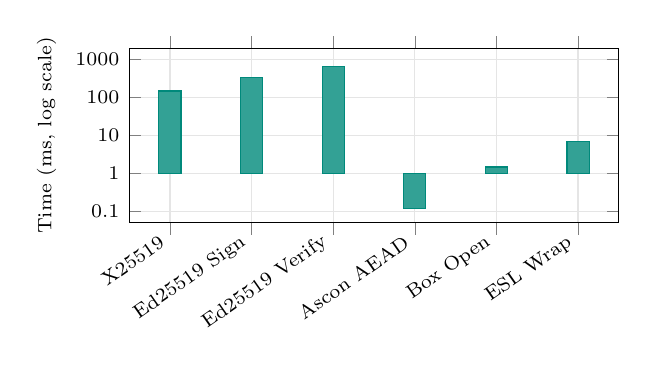
\begin{tikzpicture}
\begin{axis}[
    width=7.8cm,
    height=3.8cm,
    ybar,
    bar width=8pt,
    ylabel={Time (ms, log scale)},
    ylabel style={font=\scriptsize},
    ymode=log,
    log basis y={10},
    symbolic x coords={X25519,Ed25519 Sign,Ed25519 Verify,Ascon AEAD,Box Open,ESL Wrap},
    xtick=data,
    x tick label style={rotate=35,anchor=east,font=\scriptsize},
    ytick={0.1,1,10,100,1000},
    yticklabels={0.1,1,10,100,1000},
    y tick label style={font=\scriptsize},
    grid=major,
    grid style={gray!20},
    ymin=0.05,
    ymax=2000,
]
\addplot[fill=tealPlot!80, draw=tealPlot] coordinates {(X25519,148.0) (Ed25519 Sign,332.3) (Ed25519 Verify,663.3) (Ascon AEAD,0.12) (Box Open,1.47) (ESL Wrap,7.0)};
\end{axis}
\end{tikzpicture}%
}
\caption{Hardware-measured per-fragment stage latencies on ESP32 at 160\,MHz ($N\ge50$). Ed25519 dominates receive cost; symmetric primitives are $3$--$4$ orders of magnitude cheaper.}
\label{fig:stage_timing}
\end{figure}

\section{Discussion and Threats to Validity}

\paragraph{Stage Timing Decomposition and Software vs.\ Physical Latency.} On transmit, Ed25519 signing ($332.3$\,ms) accounts for $90.9\%$ of $\text{submit}\rightarrow\text{pulse}$ ($365.5$\,ms), leaving $\approx 33.2$\,ms for compression, Ascon-128, outer box, and framing. On receive, Ed25519 verification ($663.3$\,ms), outer box open ($1.47$\,ms), and Ascon decrypt ($0.33$\,ms) account for $665.1$\,ms of $\text{rx\_cb}\rightarrow\text{accept}$ ($727.3$\,ms), leaving $\approx 62.2$\,ms for ESL checks, decompression, and queueing. Likewise, the one-way $\text{edge}\rightarrow\text{rx\_cb}$ median of $26.6$--$27.2$\,ms is $\approx 10\times$ the $2.032$--$2.528$\,ms physical airtime, measuring software driver and callback dispatch rather than RF propagation. Software latency dominates physical airtime.

\paragraph{Role of the Shannon Entropy Check.} While Fig.~\ref{fig:verified_panels}c plots pooled-byte Shannon entropy ($6.787$\,bits/byte for Mode-A plaintext vs.\ $7.344$\,bits/byte for the CEE-PEW ESL body), we treat this solely as a sanity check against framing errors (such as zero-filled buffers). High Shannon entropy never proves cryptographic security. Entropy checks verify framing integrity only; our security claims rest on the RFC/Ascon known-answer vectors, AD-bound authentication, and $100$-vector replay rejection in Table~\ref{tab:hex_comparison}.

\paragraph{Threats to Validity.} (1)~\textit{Construct:} sync-wire stamps measure software driver boundaries, and $\Delta_{\text{heap,app}}=0$\,B scopes application allocations only. (2)~\textit{Internal:} Core~0 UI rendering contends realistically with Core~1 during timing runs. (3)~\textit{External:} measurements come from a single ESP32 DevKit~v1 board pair at $20$\,cm LOS on Channel~1; multi-board variance, longer distances, and controlled RF interference require dedicated future campaigns. (4)~\textit{Conclusion:} cluster bootstrapping accounts for shared-channel correlation, and $100/100$ host replay rejection bounds the host harness failure rate below $\approx 3\%$ at $95\%$ confidence without claiming an OTA failure rate.

\section{Applications and Future Work}\label{sec:future}\label{sec:swarm}
\textit{CEE-PEW Lite} ($105$\,B wire frame, $27.0$\,ms, $\approx 2.1$\,KB/s) targets periodic off-grid industrial telemetry~\cite{montiel2026,urazayev2023}, whereas \textit{CEE-PEW Full} ($187$\,B shipping frame, $727.3$\,ms RX) targets infrequent high-value commands and multi-agent swarm coordination~\cite{caniago2026} where per-fragment Ed25519 signatures prevent a compromised follower from forging coordinator broadcasts. Future work prioritizes several concrete developments. First, we plan to migrate BLE pairing to \textbf{SPAKE2+ (RFC~9383)}~\cite{rfc9383} with Tamarin verification~\cite{vanderlinden2023}. Second, we will benchmark a constant-time \textbf{32-bit radix-$2^{25.5}$ Ed25519 implementation} on DevKit~v1 and deploy our 4-slot \textbf{Verification Cache}. Third, we will add an \textbf{application-layer ACK/NACK protocol} for end-to-end delivery confirmation. Fourth, we will flash and run a $5$\,h hardware regression test on \texttt{FIX-BLE-CTX-RELEASE}. Fifth, we plan to fix the 9-channel hopping shift defect and conduct \textbf{OTA replay-injection and controlled interference campaigns} across multiple board pairs and distances. Finally, we will audit emitted Xtensa assembly for CVE-2025-12888 timing leaks~\cite{cve2025_12888}.

\section{Conclusion}
CEE-PEW secures connectionless ESP-NOW edge links on dual-core ESP32 nodes ($<$US\$28/pair) via sequential BLE-to-ESP-NOW radio handoff, in-band X25519 PFS re-keying, and AD-bound Ascon-128 v1.2 encryption. Outer XSalsa20-HMAC-128 filtering and a 64-bit post-authentication sliding replay bitmap operate within a $187$\,B shipping wire frame ($105$\,B in Lite mode) and zero application heap allocation ($\Delta_{\text{heap,app}}=0$\,B). Our evaluation rejects 100/100 host replay and 24/24 header-tamper vectors, isolates the $663.3$\,ms Ed25519 bottleneck to 64-bit-limb TweetNaCl emulation, quantifies the $\approx 8$\,pp gap between MAC-ACK completion and application reassembly, and demonstrates via controlled ablation that Hamming(15,11) FEC corrects zero errors over clean 802.11 FCS links. All findings reflect real hardware.

\section*{Acknowledgment}
The authors used AI tools for language editing and clarity. All technical content, firmware, and measurements were verified by the authors.

{\footnotesize\begin{thebibliography}{99}
\setlength{\itemsep}{0pt}\setlength{\parskip}{0pt}
\bibitem{montiel2026} M.~N.~Montiel~Torres, ``ESP-NOW vs.\ WiFi: An analysis of temporal determinism in high-frequency industrial telemetry,'' in \textit{Proc.\ 55 JAIIO}, 2026.
\bibitem{espressif_espnow} Espressif Systems, ``ESP-NOW User Guide (v1.0 and v2.0 Frame Formats),'' \textit{ESP-IDF Programming Guide v6.0}, 2025.
\bibitem{espressif_espnow_component} Espressif Systems, ``ESP-NOW Component User Guide: AES128-CCM Data Encryption, v2.5.2,'' GitHub, 2024.
\bibitem{cujilema2023} J.~A.~Cujilema~Paguay \textit{et al.}, ``Secure home automation system based on ESP-NOW mesh network, MQTT and Home Assistant platform,'' \textit{IEEE Latin America Trans.}, vol.~21, no.~7, pp.~781--789, 2023.
\bibitem{caniago2026} D.~P.~Caniago \textit{et al.}, ``Swarm robot communication using ESP-NOW mesh protocol for multi-agent coordination in indoor navigation,'' \textit{J.\ Europ{\'e}en des Syst{\`e}mes Automatis{\'e}s}, vol.~59, no.~5, pp.~1263--1274, 2026.
\bibitem{espressif_issue15179} Espressif Systems, ``ESP-NOW authentication and vulnerability,'' \textit{esp-idf GitHub Issue \#15179}, 2025 (open; last activity Jan.\ 2025).
\bibitem{nozomi2024} Nozomi Networks Labs, ``Flaws in Espressif ESP-NOW Allow Attackers to Replay Communications (CVE-2024-42483, CVE-2024-42484),'' disclosed Sept.\ 10 2024 (NVD/CISA Sept.\ 12 2024), fixed in v2.5.2 (commits 4e30db50+b03a1b45).
\bibitem{guardianair2024} Nozomi Networks, ``Guardian Air: Wireless intrusion detection documentation, ESP-NOW protocol identification via Espressif OUI,'' Nozomi Networks Documentation, 2024.
\bibitem{nvd_cve42483} National Vulnerability Database (NVD), ``CVE-2024-42483: Espressif esp-now Component Replay Vulnerability (Fixed in v2.5.2, commits 4e30db50+b03a1b45),'' NIST, Sept.\ 12 2024. Available: \url{https://nvd.nist.gov/vuln/detail/CVE-2024-42483}, accessed Oct.\ 2026.
\bibitem{securepair2026} toggio, ``SecurePair: Cryptographically secure pairing and communication (X25519 + AES-256-GCM) over ESP-NOW and LoRa,'' GitHub Repository, 2026.
\bibitem{setiawan2021} F.~B.~Setiawan and Magfirawaty, ``Securing data communication through MQTT protocol with AES-256 encryption algorithm CBC mode on ESP32-based smart homes,'' in \textit{Proc.\ IEEE ICIC}, 2021, pp.~166--170.
\bibitem{amirkhanova2026} G.~Amirkhanova \textit{et al.}, ``A lightweight, end-to-end encrypted data pipeline for IIoT: An AES-GCM implementation for ESP32, MQTT, and Raspberry Pi,'' \textit{Information}, vol.~17, no.~1, art.~33, 2026.
\bibitem{rfc7748} A.~Langley, M.~Hamburg, and S.~Turner, ``Elliptic Curves for Security,'' IETF RFC 7748, Jan.\ 2016.
\bibitem{rfc5869} H.~Krawczyk and P.~Eronen, ``HMAC-based Extract-and-Expand Key Derivation Function (HKDF),'' IETF RFC 5869, May 2010.
\bibitem{rfc8439} Y.~Nir and A.~Langley, ``ChaCha20 and Poly1305 for IETF Protocols,'' IETF RFC 8439, June 2018.
\bibitem{dobraunig2021} C.~Dobraunig, M.~Eichlseder, F.~Mendel, and M.~Schl{\"a}ffer, ``Ascon v1.2: Lightweight authenticated encryption and hashing,'' \textit{J.\ Cryptology}, vol.~34, no.~3, art.~33, 2021.
\bibitem{nist_ascon2025} M.~S{\"o}nmez~Turan, K.~A.~McKay, D.~Chang, J.~Kang, and J.~Kelsey, ``Ascon-Based Lightweight Cryptography Standards for Constrained Devices,'' \textit{NIST Special Publication 800-232}, Aug.\ 2025.
\bibitem{bernstein2012} D.~J.~Bernstein, N.~Duif, T.~Lange, P.~Schwabe, and B.-Y.~Yang, ``High-speed high-security signatures,'' \textit{J.\ Cryptographic Eng.}, vol.~2, no.~2, pp.~77--89, 2012.
\bibitem{donenfeld2017} J.~A.~Donenfeld, ``WireGuard: Next generation kernel network tunnel,'' in \textit{Proc.\ NDSS}, 2017.
\bibitem{atul2026} Atul, Vivek Shukla, M.~K.~Das, Varun Shukla, and D.~Mishra, ``A reproducible security--performance benchmark protocol for lightweight AEAD on resource-constrained IoT nodes,'' \textit{IACR Cryptology ePrint Archive}, Paper 2026/1882, 2026 (Preprint, protocol proposal without hardware results).
\bibitem{oryx_esp32} Oryx Embedded, ``Crypto Benchmark on ESP32 MCU (CycloneCRYPTO at 240\,MHz),'' Live benchmark web page, accessed Oct.\ 2026.
\bibitem{urazayev2023} D.~Urazayev, A.~Eduard, M.~Ahsan, and D.~Zorbas, ``Indoor performance evaluation of ESP-NOW,'' in \textit{Proc.\ IEEE SIST}, 2023, pp.~1--5.
\bibitem{meshtastic2026} Meshtastic, ``Meshtastic: An open-source, off-grid mesh networking project,'' Project documentation, 2026. Available: \url{https://meshtastic.org}, accessed Oct.\ 2026.
\bibitem{albrecht2021} M.~R.~Albrecht, J.~Blasco, R.~B.~Jensen, and L.~Marekov{\'a}, ``Mesh messaging in large-scale protests: Breaking Bridgefy,'' in \textit{Proc.\ CT-RSA}, LNCS vol.~12704, Springer, 2021, pp.~375--398.
\bibitem{lin2004} S.~Lin and D.~J.~Costello, \textit{Error Control Coding}, 2nd~ed.\ Upper Saddle River, NJ: Prentice Hall, 2004.
\bibitem{yin2020} Z.~Yin \textit{et al.}, ``SafetyNet: Interference protection via transparent PHY layer coding,'' in \textit{Proc.\ IEEE ICDCS}, 2020, pp.~267--277.
\bibitem{vontschirschnitz2021} M.~von~Tschirschnitz, L.~Peuckert, F.~Franzen, and J.~Grossklags, ``Method confusion attack on Bluetooth pairing,'' in \textit{Proc.\ IEEE S\&P}, 2021, pp.~1332--1347.
\bibitem{jangid2023} M.~K.~Jangid, Y.~Zhang, and Z.~Lin, ``Extrapolating formal analysis to uncover attacks in Bluetooth passkey entry pairing,'' in \textit{Proc.\ NDSS}, 2023.
\bibitem{vanderlinden2023} T.~Claverie, G.~Avoine, S.~Delaune, and J.~Lopes~Esteves, ``Tamarin-based analysis of Bluetooth uncovers two practical pairing confusion attacks,'' in \textit{Proc.\ ESORICS 2023}, LNCS vol.~14346, Springer, 2023, pp.~100--119.\ doi:10.1007/978-3-031-51479-1\_6.
\bibitem{cve2025_12888} wolfSSL Inc.\ / NVD, ``CVE-2025-12888: X25519 Constant-Time Compiler Issue on Xtensa-Based ESP32 Chips,'' Dec.\ 2025. Available: \url{https://nvd.nist.gov/vuln/detail/CVE-2025-12888}, accessed Oct.\ 2026.
\bibitem{rfc9383} W.~Ladd and B.~Kaduk, ``SPAKE2+, an Augmented Password-Authenticated Key Exchange (PAKE) Protocol,'' IETF RFC 9383, Sept.\ 2023.
\bibitem{hamming1950} R.~W.~Hamming, ``Error detecting and error correcting codes,'' \textit{Bell Syst.\ Tech.\ J.}, vol.~29, no.~2, pp.~147--160, 1950.\ doi:10.1002/j.1538-7305.1950.tb00463.x.
\bibitem{efron1979bootstrap} B.~Efron, ``Bootstrap methods: another look at the jackknife,'' \textit{Ann.\ Statist.}, vol.~7, no.~1, pp.~1--26, 1979.
\end{thebibliography}
\ifanonymous
\else
\par\vspace{2pt}\noindent\textit{Source code, Lua dissector, and PCAP artifacts:} \url{https://github.com/R1sh1m/CEEPEW}
\fi
}

\end{document}
